\documentclass[preprint,12pt]{elsarticle}

\usepackage[utf8]{inputenc}
\usepackage[T1]{fontenc}
\usepackage{lmodern}
\usepackage[margin=1in]{geometry}
\usepackage{graphicx}
\usepackage{booktabs}
\usepackage{amsmath}
\usepackage[colorlinks=true,linkcolor=blue,citecolor=blue,urlcolor=blue]{hyperref}
\usepackage{setspace}
\usepackage{float}
\usepackage{lineno}
\onehalfspacing

\journal{Journal of Hydrology: Regional Studies}
\biboptions{authoryear,round}

\begin{document}

\begin{frontmatter}

\title{Climate-Driven River--Coastal Connectivity Across Puerto Rico: Multi-Basin Evidence from Hydrologic and Satellite Observations}

\author[wku]{Somnath Luitel\corref{cor1}}
\ead{somnath.luitel@topper.wku.edu}
\author[wku]{Manmeet Singh}

\cortext[cor1]{Corresponding author}
\affiliation[wku]{organization={AI Research Lab, Department of Earth, Environmental, and Atmospheric Sciences, Western Kentucky University},
            city={Bowling Green}, state={KY}, country={USA}}

\begin{abstract}
Puerto Rico's coastal ecosystems receive river-borne pulses of freshwater, sediment, and nutrients driven by island rainfall variability, yet no study has connected the full chain --- climate driver, river discharge, and coastal ocean-color response --- across multiple watersheds using a continuous multi-decadal record and an explainable machine learning framework. We assembled discharge (up to 66 years), precipitation, and satellite chlorophyll-a records for 10 Puerto Rico watersheds spanning every coast, using only publicly available government and satellite data. A two-stage modeling framework tested (1) whether local drought conditions (Standardized Precipitation Index, SPI), rather than the El Ni\~no--Southern Oscillation (ENSO), explain discharge variability, and (2) whether a discharge signal propagates detectably to coastal chlorophyll-a. Stage 1 was confirmed across all 10 basins: an ElasticNet model using SPI and seasonality explains 32--74\% of out-of-sample discharge anomaly variance (permutation test, $p=0.005$ for the primary basin), with 1-month drought conditions the dominant driver by SHAP attribution. Stage 2 found a discharge--chlorophyll linkage with strong statistical support in 2 of 7 testable basins ($p=0.005$ for both), and weak/mixed evidence in 2 more, concentrated offshore rather than at the river mouth in most cases. Basin-to-basin variation in Stage 2 skill was not explained by drainage area or discharge magnitude, but was partly explained by inter-satellite-sensor data-merging quality --- a methodological confound we identified and directly tested by reprocessing affected basins with single-sensor data, confirming the effect in 2 of 3 cases. These results provide multi-basin, explainable-ML evidence for climate-driven river-to-coast linkages in a tropical Caribbean setting and identify concrete data-quality considerations for future satellite-based coastal monitoring in small-island systems.
\end{abstract}

\begin{keyword}
river discharge \sep coastal chlorophyll-a \sep explainable machine learning \sep Standardized Precipitation Index \sep Puerto Rico \sep multi-basin hydrology
\end{keyword}

\end{frontmatter}

\linenumbers

\section{Introduction}

Small tropical islands present a distinctive hydroclimatic setting in which short, steep watersheds respond rapidly to rainfall variability and the resulting river discharge reaches the coast within a short distance and time, creating a potentially tight coupling between terrestrial climate variability and coastal ecosystem state. Puerto Rico, situated in the northeastern Caribbean, exemplifies this setting and is subject to substantial interannual rainfall variability. Contrary to a common assumption in Caribbean climate studies, this variability is not primarily controlled by the El Ni\~no--Southern Oscillation: \citet{torresvalcarcel2018enso} found only a weak, spatially inconsistent ENSO signal in Puerto Rico rainfall and drought across all climate regions of the island, with local and regional factors playing a larger role. Two halves of the resulting climate--river--coast chain have nonetheless been studied only separately in Puerto Rico to date. At the island scale, \citet{trossitorres2025precipitation} characterized 1990--2022 precipitation trends and their relationship to reservoir levels and river discharge, finding declining precipitation alongside contradictory reservoir and streamflow trends attributable to factors beyond precipitation alone. Separately, \citet{hernandez2020hurricanes} used VIIRS satellite imagery to quantify acute coastal water-quality responses --- chlorophyll-a and the diffuse attenuation coefficient $K_d(490)$ --- to the extreme discharge pulses generated by Hurricanes Irma and Maria in 2017. Neither study connects the full chain across a continuous, multi-year record, nor tests whether any such linkage is a general feature of Puerto Rico watersheds or an idiosyncrasy of a single basin or a small number of extreme events, leaving open the question this study addresses.

The coastal side of this chain matters ecologically as well as methodologically. Chlorophyll-a is the most widely used proxy for phytoplankton biomass in aquatic systems, and its concentration integrates the combined influence of nutrient availability, light, and mixing on primary production \citep{boyer2009phytoplankton}. Persistently elevated chlorophyll-a signals eutrophication and an elevated risk of harmful algal blooms, while depressed values can indicate light or nutrient limitation; because it is comparatively simple and inexpensive to measure relative to direct phytoplankton enumeration, chlorophyll-a has become the default indicator in coastal water-quality monitoring programs, including those targeted by satellite ocean-color missions. A river-discharge-driven chlorophyll-a response is therefore not merely a statistical curiosity: it reflects a real pathway by which terrestrial climate variability propagates into coastal primary production, nutrient loading, and, ultimately, ecosystem condition — the kind of linkage that management and monitoring programs in small tropical islands need to anticipate rather than discover after the fact.

Beyond Puerto Rico, remote-sensing studies of river-influenced coastal chlorophyll-a have generally taken one of two forms: basin-specific empirical retrieval models tuned to a single estuary using in-situ and satellite data together, such as the Pearl River Estuary random-forest retrieval framework of \citet{yuan2022spatiotemporal}, or broader mapping studies of discharge-chlorophyll covariation over large shelf regions and long time series, such as \citet{auricht2022mapping}, who additionally showed that the lag between peak discharge and the coastal chlorophyll response is itself a variable worth characterizing empirically rather than assuming. A separate strand of work has focused on the reliability of the satellite chlorophyll-a retrieval itself: \citet{holbach2025chlorophyll} recently demonstrated, in the optically complex coastal waters of Denmark, that a single globally calibrated satellite chlorophyll-a algorithm can carry substantial regional bias, and that spatially resolved recalibration meaningfully improves agreement with in-situ observations. What is comparatively rare across this literature is a study design that (a) spans multiple independent watersheds within one climate region, explicitly testing whether a detected discharge-chlorophyll linkage generalizes rather than reflects one basin's idiosyncrasy, (b) uses an explainable modeling framework capable of attributing predictive skill to a specific driver and lag rather than reporting predictive accuracy alone, and (c) treats satellite data-merging quality itself as a variable to be diagnosed rather than assumed adequate --- a gap this study is designed to close, and one that connects directly to the broader machine-learning-in-hydrology literature: \citet{slater2025challenges} recently reviewed the promise and the open challenges of explainable AI applied at the scale of many catchments simultaneously, including the risk that a model's apparent skill or lack thereof reflects data quality and availability rather than the underlying physical process, a risk we treat as a central rather than incidental part of the present analysis.

We address this gap with three hypotheses. First, we hypothesize that local precipitation and drought conditions, indexed by the Standardized Precipitation Index, rather than ENSO, are the dominant driver of river discharge variability in Puerto Rico watersheds (H1), a hypothesis motivated directly by the weak ENSO teleconnection reported by \citet{torresvalcarcel2018enso}. Second, we hypothesize that a drought-driven discharge signal detectably propagates to coastal chlorophyll-a in at least some Puerto Rico watersheds, at a characteristic lag and spatial position relative to the river mouth that need not coincide with the mouth itself (H2). Third, we hypothesize that an explainable machine-learning framework can jointly quantify this predictive skill and attribute it to a specific driver and lag, and, further, can be used diagnostically to distinguish a genuine absence of a coastal linkage from a data-quality limitation in a given basin (H3). We test these hypotheses using a ten-basin dataset assembled entirely from public government and satellite sources, a two-stage explainable machine-learning framework validated with two independent cross-validation schemes and permutation-based significance testing, and a set of cross-basin diagnostics --- including a satellite data-merging confound that we identify, test directly, and partially confirm --- that we argue are broadly relevant to future satellite-based coastal monitoring studies in small-island settings.

\section{Study Area and Data}

\subsection{Study region}
Ten Puerto Rico watersheds were selected from the full USGS Puerto Rico streamgage network ($n\approx124$ active gauges), screened for (a) long, continuous daily discharge records, (b) gauges not directly downstream of a dam or reservoir, verified per-gauge by inspecting flow statistics for a regulation signature (an automated flag for a high fraction of days at a near-constant minimum flow, supplemented by manual inspection for the primary basin), and (c) geographic spread across the island's north, south, east, and west coasts (Fig.~\ref{fig:studyarea}, Table~\ref{tab:stagea}). Drainage areas range from 6.6 to 208~mi$^2$ (USGS-reported), spanning nearly an order of magnitude and allowing basin size itself to be tested as a possible explanatory variable for cross-basin variation in results (Section~4.3).

\begin{figure}[htbp]
\centering
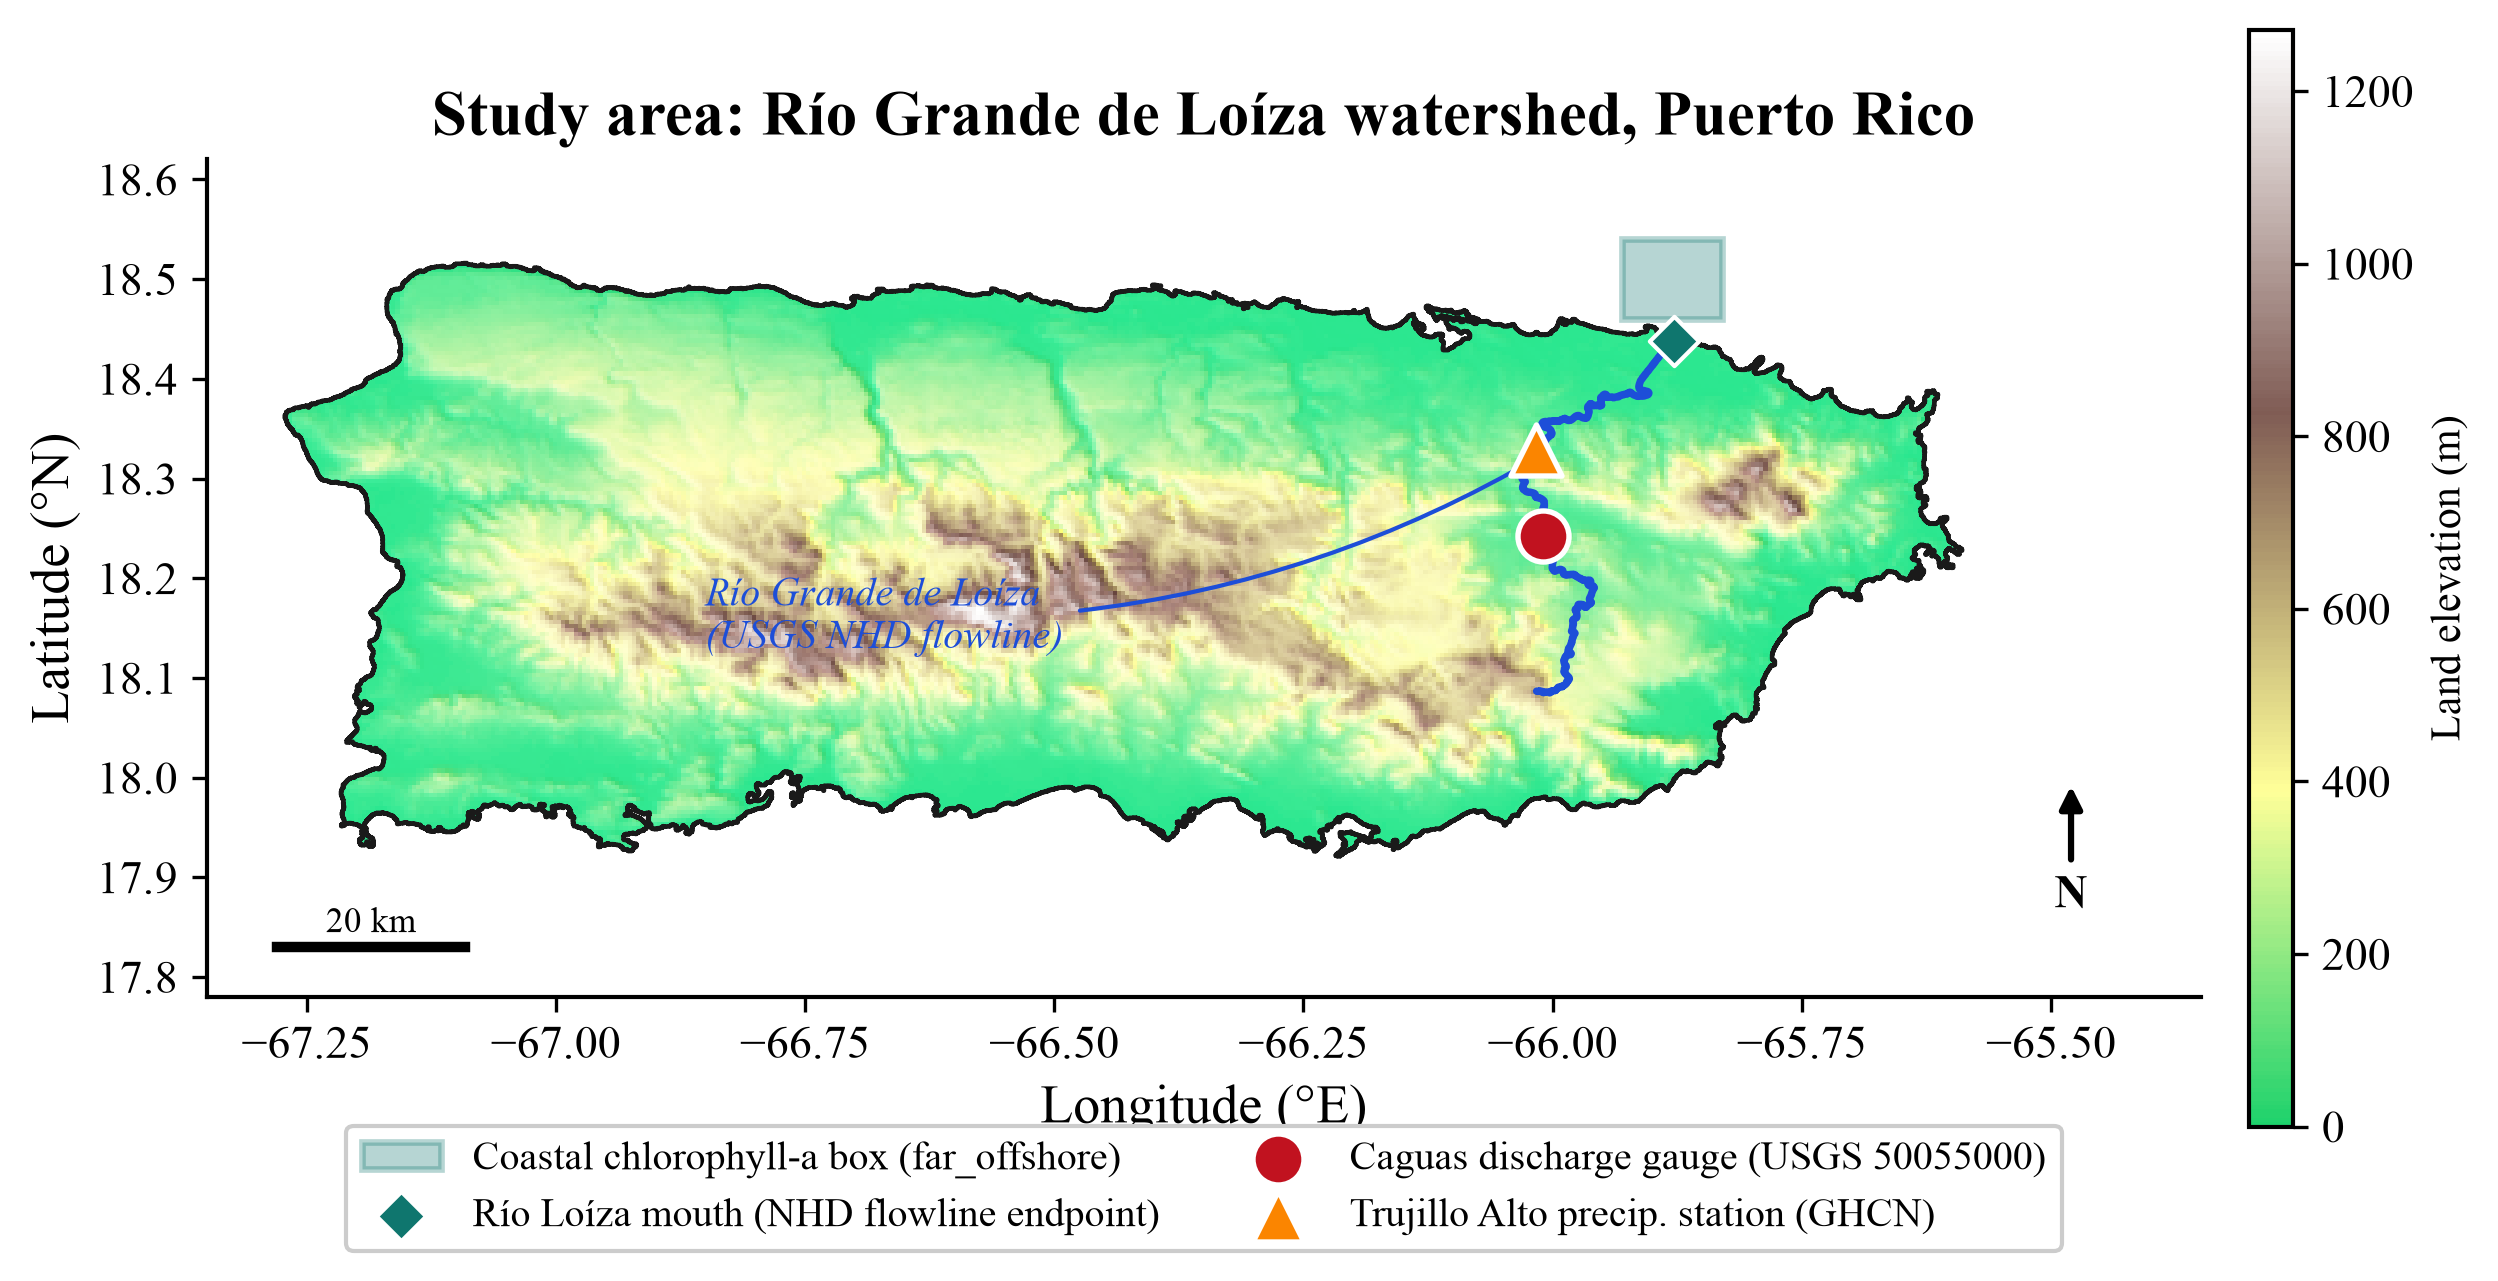
\includegraphics[width=0.85\textwidth]{../figures/08_study_area_map.png}
\caption{Study area: Río Grande de Loíza watershed, the primary study basin, showing the discharge gauge, precipitation station, USGS NHD-derived river channel, and the coastal chlorophyll-a sampling box. Land elevation is from GEBCO\_2020 (15 arc-second); the coastline is the UN OCHA COD-AB boundary, adopted after an initial Census TIGERweb boundary was found to contain a cartographic artifact connecting the mainland to Vieques and Culebra.}
\label{fig:studyarea}
\end{figure}

\subsection{Discharge data}
Daily mean discharge was obtained from the USGS National Water Information System (NWIS) public web service for each gauge's full period of record. Series were aggregated to monthly means, log-transformed to address the strong right skew characteristic of streamflow, and expressed as anomalies relative to each series' own long-term monthly climatology to isolate interannual variability from the seasonal cycle. Monthly series were reindexed to a continuous calendar prior to any rolling-window or lagged-feature computation, so that a calendar gap is represented as a missing value rather than silently causing rolling operations to bridge non-adjacent months. This is not a cosmetic detail: correcting it changed the primary basin's headline Stage~A skill from an initially reported NSE of 0.514 to the corrected value of 0.390 reported throughout this paper (Section~4.1), and we report this transparently as an illustration of the check's practical importance for any similarly constructed pipeline.

\subsection{Precipitation data and the Standardized Precipitation Index}
Daily precipitation was obtained from the NOAA Global Historical Climatology Network-Daily (GHCN-D) archive, using the nearest station to each gauge with adequate temporal coverage (within approximately 16~km, record extending to at least 2020, longest available record preferred among qualifying stations). The Standardized Precipitation Index \citep[SPI;][]{mckee1993spi} was computed following the standard multi-timescale formulation of \citet{edwards1997characteristics}, with the Gamma distribution fitting procedure of \citet{thom1958gamma}. For a given accumulation window $w$ (here $w \in \{1,3,6,12\}$ months) and calendar month $m$, let $X_{w,m}$ denote the set of $w$-month accumulated precipitation totals observed in calendar month $m$ across the record. A two-parameter Gamma distribution is fit to the non-zero values of $X_{w,m}$ by maximum likelihood \citep{thom1958gamma}, with probability density function
\begin{equation}
f(x;\alpha,\beta) = \frac{1}{\beta^{\alpha}\Gamma(\alpha)}\, x^{\alpha-1} e^{-x/\beta}, \qquad x>0,
\label{eq:gamma}
\end{equation}
where $\alpha$ and $\beta$ are the shape and scale parameters estimated separately for each calendar month. Because an accumulation window can have zero total precipitation, the cumulative probability is adjusted for the probability of zero precipitation, $q = n_0/n$ (the fraction of zero-valued observations in that calendar month):
\begin{equation}
H(x) = q + (1-q)\,G(x;\alpha,\beta),
\label{eq:spicdf}
\end{equation}
where $G(x;\alpha,\beta)$ is the Gamma cumulative distribution function. The resulting probability $H(x)$ is transformed to a standard normal quantile via the inverse standard normal cumulative distribution function $\Phi^{-1}$ (the probit function):
\begin{equation}
\mathrm{SPI} = \Phi^{-1}\big(H(x)\big).
\label{eq:spi}
\end{equation}
This yields a dimensionless, approximately normally distributed index in which negative values indicate below-normal precipitation (incipient or ongoing meteorological drought) and positive values indicate above-normal precipitation, directly comparable across accumulation windows and calendar months. The SPI is computed independently at each of the four accumulation windows used here, giving four distinct predictors reflecting drought conditions accumulated over the preceding 1, 3, 6, and 12 months respectively.

\subsection{Satellite chlorophyll-a and inter-sensor merging}
Coastal chlorophyll-a was obtained from two NOAA CoastWatch ERDDAP-hosted ocean-color products: a legacy MODIS-Aqua monthly composite (2003--2022) and the current VIIRS/S-NPP science-quality monthly product (2012--present). Because no single sensor spans the full discharge record, and switching sensors introduces retrieval-algorithm bias, the two products were merged via a log-log linear bias correction fit on their overlap period (2012--2022):
\begin{equation}
\log(\mathrm{Chl}_{\mathrm{MODIS}}) = a + b \log(\mathrm{Chl}_{\mathrm{VIIRS}}),
\label{eq:biascorrection}
\end{equation}
with $a$ and $b$ fit by ordinary least squares on the overlap-period matchups, applied to VIIRS values only for the period after MODIS coverage ends (no double-correction within the overlap window). The coefficient of determination of this fit, $R^2$, varied substantially by basin (0.11--0.73; Table~\ref{tab:stageb}) and is treated in Section~4.3 not merely as a diagnostic of fit quality but as a candidate explanatory variable for cross-basin differences in Stage~2 skill, in the same spirit as the regional recalibration approach of \citet{holbach2025chlorophyll}.

\subsection{Ancillary data}
Sea-surface temperature (NOAA OISST v2.1, daily, 0.25$^{\circ}$ resolution) and 10~m wind speed (NCEP/NCAR Reanalysis, monthly, approximately 1.9$^{\circ}$ resolution) were tested as additional Stage~2 covariates for a subset of basins (Section~4.2), motivated by the expectation that coastal chlorophyll-a variability is influenced by thermal stratification and wind-driven mixing in addition to riverine nutrient and freshwater input.

\subsection{River mouth determination}
For each basin, the coastal river mouth was located using the USGS National Hydrography Dataset (NHD) flowline layers, taking the point on that river's named flowline geometrically closest to the true coastline. This geometric approach was adopted after an initial directional heuristic (assuming the river mouth is the northernmost flowline point) was found during development to fail for any river not flowing predominantly north --- a category that includes several of the ten basins studied here. Where NHD lacked a named reach for a given river (2 of 12 rivers attempted), OpenStreetMap's Overpass API was used as a fallback and, where both sources were available for cross-checking, agreed closely with the NHD-derived location.

\subsection{Coastline and elevation reference data}
The Puerto Rico coastline boundary used throughout was obtained from UN OCHA's Common Operational Dataset for Administrative Boundaries (COD-AB, 2019). An initial boundary obtained from the U.S. Census TIGERweb service was found, on inspection, to contain a cartographic dissolve artifact --- a spurious land connection between the mainland and the islands of Vieques and Culebra --- and was replaced with the higher-resolution OCHA product (17,243 coastline vertices for the mainland alone). Elevation and bathymetry (GEBCO\_2020, 15 arc-second resolution) were used for contextual mapping only and did not inform any hydrological delineation.

\section{Methods}

\subsection{Modeling framework}
A two-stage framework was used throughout (Fig.~\ref{fig:flowchart}). In Stage~A (climate~$\rightarrow$~discharge), the predictors are SPI at the four accumulation windows described in Section~2.3, raw monthly precipitation, sine- and cosine-encoded calendar month (to represent seasonality without imposing an arbitrary reference month), and the lag-1 discharge anomaly; the target is the log discharge anomaly for the current month. In Stage~B (discharge~$\rightarrow$~coastal chlorophyll), the predictors are the discharge anomaly at lags 0 through 3 months, the 3-month SPI, and calendar seasonality, optionally augmented with sea-surface temperature and wind-speed anomalies (Section~4.2); the target is the log chlorophyll-a anomaly within an empirically selected coastal sampling box (Section~3.2).

\begin{figure}[htbp]
\centering
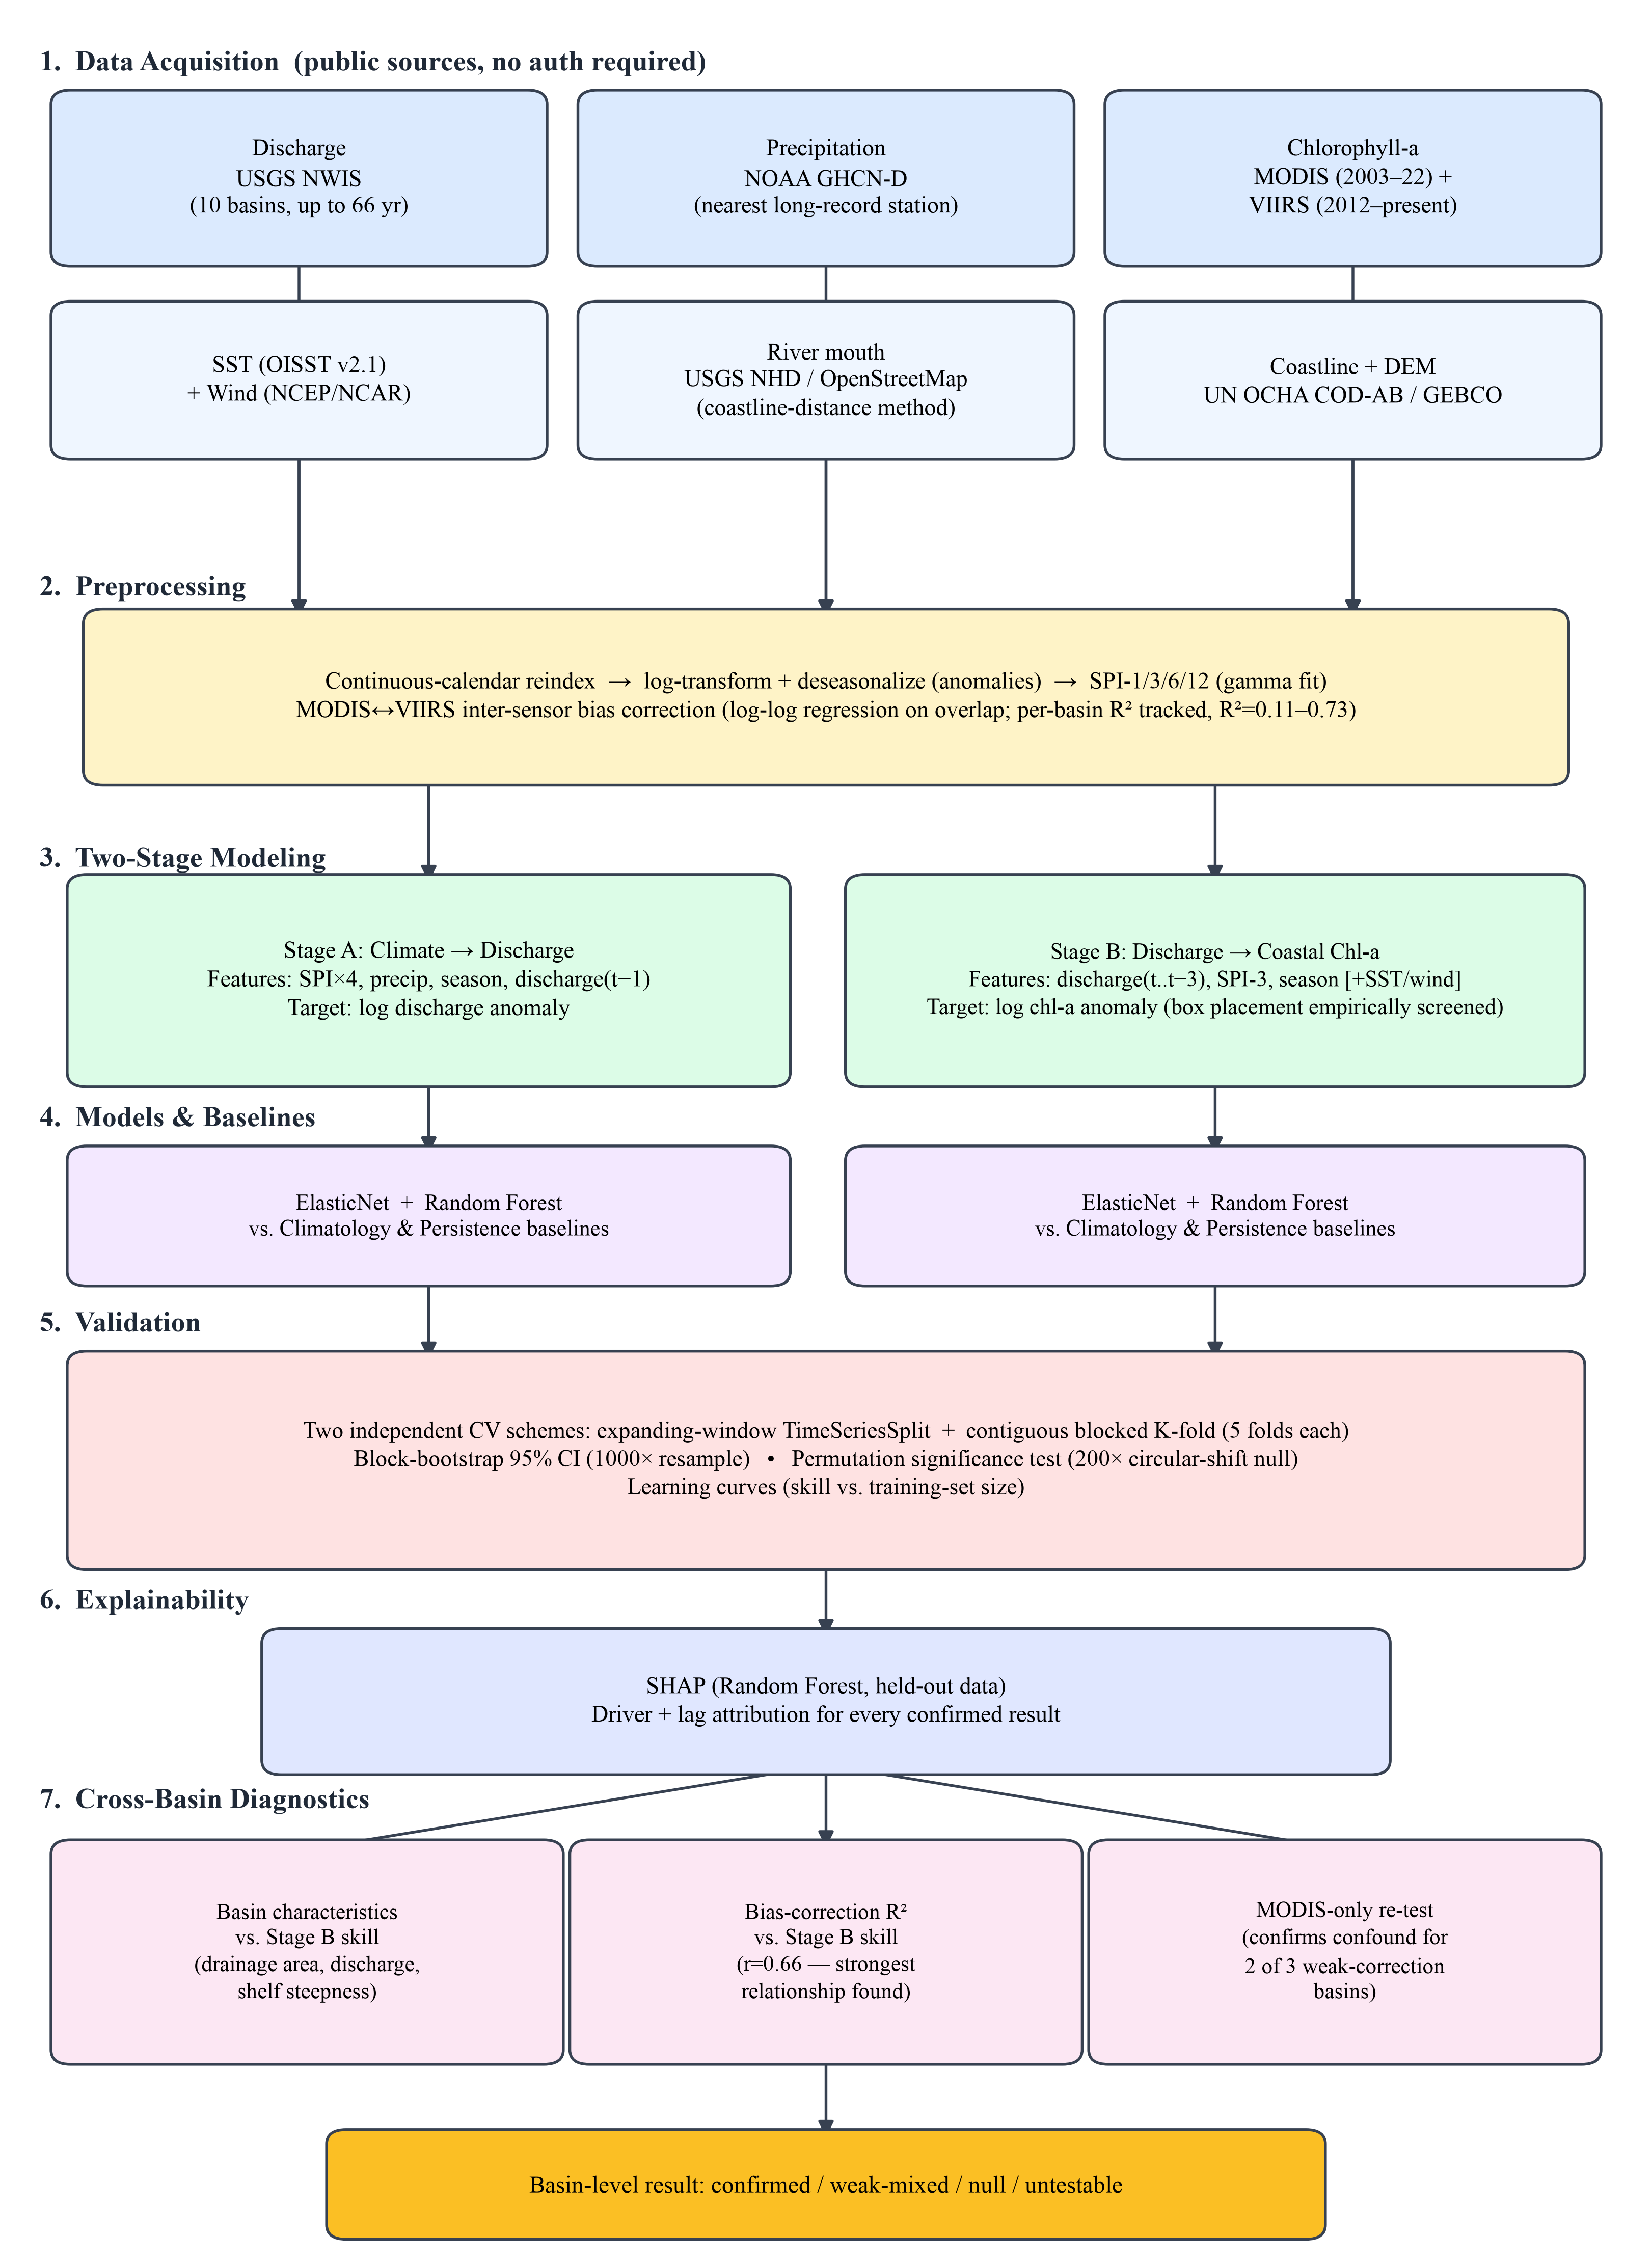
\includegraphics[width=0.9\textwidth]{../figures/22_methodology_flowchart.png}
\caption{Methodology flowchart: data acquisition, preprocessing, the two-stage modeling framework, validation protocol, explainability, and cross-basin diagnostics.}
\label{fig:flowchart}
\end{figure}

\subsection{Coastal box placement}
For each basin, two candidate coastal sampling boxes were tested: one centered on the river mouth, and one offset radially outward by approximately 9~km, with the offset direction computed from the island's geographic centroid through the mouth so that it is well defined regardless of which coast a given basin drains to. Placement was decided empirically per basin via a lag-0-through-3 cross-correlation screen between discharge anomaly and chlorophyll-a anomaly, computed prior to full model validation; no single placement rule was assumed to generalize across basins a priori. This proved to be the correct approach rather than a formality: 5 of 7 basins screened favored the offshore box, but 2 (Culebrinas, Guanajibo) instead favored the mouth-centered box, a genuine cross-basin difference discussed further in Section~5.2.

\subsection{Models and baselines}
Two models were fit at each stage: ElasticNet, a linear model with combined L1/L2 regularization whose penalty strength was selected via nested time-series cross-validation, and Random Forest, configured with a shallow maximum depth (4--6) to match the available sample size. Two baselines were evaluated alongside every model: a climatological baseline that predicts the anomaly's own long-term mean (equivalently, zero, since the target is already expressed as an anomaly), and a persistence baseline that predicts the prior month's observed value. Model complexity was deliberately kept modest relative to the deep-learning approaches common in the broader chlorophyll remote-sensing literature, which are typically applied to daily or higher-frequency records with substantially larger sample sizes than are available here (monthly records, with sample sizes in the low hundreds at each basin); this choice is supported empirically, not merely asserted, by the observation that ElasticNet matched or exceeded Random Forest at every basin and stage tested (Tables~\ref{tab:stagea}--\ref{tab:stageb}).

\subsection{Cross-validation}
Two independent folding schemes were used for every cross-validated result reported: an expanding-window scheme (scikit-learn's \texttt{TimeSeriesSplit}, 5 folds), in which the training set grows chronologically and the model is always evaluated on data strictly after its training window, and a contiguous blocked $K$-fold scheme (5 folds, no shuffling), in which the record is divided into five chronological blocks and each is held out in turn. Random or shuffled $K$-fold cross-validation was deliberately not used at any point, since it would allow information to leak across autocorrelated neighboring months and would overstate skill.

\subsection{Evaluation metrics}
Nash--Sutcliffe Efficiency \citep[NSE;][]{nash1970river} is the primary skill metric used throughout, computed on held-out data only:
\begin{equation}
\mathrm{NSE} = 1 - \frac{\sum_{i=1}^{n}(O_i - P_i)^2}{\sum_{i=1}^{n}(O_i - \bar{O})^2},
\label{eq:nse}
\end{equation}
where $O_i$ and $P_i$ are the observed and predicted values and $\bar{O}$ is the mean of the observed values over the evaluation period. NSE equals 1 for a perfect model, 0 for a model no better than predicting the mean, and is unbounded below. Kling--Gupta Efficiency \citep[KGE;][]{gupta2009decomposition} is reported as a secondary, diagnostic metric:
\begin{equation}
\mathrm{KGE} = 1 - \sqrt{(r-1)^2 + (\alpha-1)^2 + (\beta-1)^2},
\label{eq:kge}
\end{equation}
where $r$ is the Pearson correlation between observed and predicted values, $\alpha = \sigma_P/\sigma_O$ is the ratio of predicted to observed standard deviation (a variability-error term), and $\beta = \mu_P/\mu_O$ is the ratio of predicted to observed mean (a bias term). We found $\beta$ to be numerically unstable for the zero-centered anomaly series used throughout this study, since $\mu_O$ is close to zero by construction; KGE is therefore reported for completeness but interpreted with this caveat, and Spearman rank correlation is additionally reported as a metric less sensitive to this instability. Root-mean-square error and mean absolute error are reported in native (log-anomaly) units for interpretability alongside the skill scores.

\subsection{Uncertainty and significance}
Block-bootstrap 95\% confidence intervals (1000 resamples, drawn as contiguous 6-month blocks to respect the autocorrelation present in monthly climate and ocean-color data) were computed for final-holdout NSE. To test whether observed skill exceeds what would be expected by chance --- a stricter test than simply exceeding the climatology or persistence baselines --- a permutation test was used: the target series was circularly shifted by a random offset, which preserves its own autocorrelation structure while breaking its true temporal alignment with the predictor set, across 200 independent realizations; the full modeling pipeline was refit on each shifted realization, and an empirical $p$-value was computed as the fraction of the resulting null-distribution NSE values that met or exceeded the observed NSE.

\subsection{Learning curves}
To assess whether reported skill is stable with respect to training-set size, rather than an artifact of a particular amount of training data, held-out NSE was recomputed while incrementally increasing the training set from approximately 15\% to 100\% of its full chronological extent, always taking the earliest-available data first so that no future information enters the training set at any point, for both basins with a confirmed Stage~2 result.

\subsection{Explainability}
SHAP \citep[SHapley Additive exPlanations;][]{lundberg2017unified} values, computed from the fitted Random Forest on held-out data, were used at both stages to attribute predictive skill to specific input features and, through the set of lagged discharge features used in Stage~B, to specific time lags between discharge and the coastal chlorophyll response. Because SHAP decomposes each individual prediction into additive per-feature contributions, it provides a physically interpretable answer to \emph{which} driver and \emph{what} lag underlie a given result, not merely whether the model predicts well.

\section{Results}

\subsection{Stage A: climate-driven discharge variability generalizes across basins}
All 10 tested basins showed ElasticNet clearly exceeding both baselines (Table~\ref{tab:stagea}; NSE range 0.321--0.735, median 0.505). The primary basin (Río Grande de Loíza) achieved NSE~=~0.390 on a held-out 2013--2026 test period, formally significant against a circular-shift permutation null ($p=0.005$, $n=200$; Fig.~\ref{fig:permutation}). A learning-curve analysis (Fig.~\ref{fig:learning}) showed this result to be stable rather than an artifact of a particular training window: held-out skill rose smoothly with training-set size and plateaued at approximately two-thirds of the available data, consistent with a converged relationship for which additional data collection would not obviously change the conclusion. SHAP attribution identified the 1-month SPI as the dominant predictor at every basin examined in detail, with contribution decaying smoothly across the longer accumulation windows --- a physically coherent signature of fast basin hydrological response consistent with the short, steep topography characteristic of Puerto Rico watersheds. This finding supports H1 and is inconsistent with an ENSO-driven framing of Puerto Rico discharge variability, corroborating \citet{torresvalcarcel2018enso} at the level of a downstream hydrological variable rather than rainfall alone.

\begin{table}[htbp]
\centering
\caption{Basin characteristics and Stage A results, all 10 basins tested.}
\label{tab:stagea}
\small
\begin{tabular}{lrrrrl}
\toprule
Basin & Drainage area (mi$^2$) & Record & $n$ (mo.) & NSE$_{\mathrm{ElasticNet}}$ & Verdict \\
\midrule
Loíza (primary) & 89.8 & 1969--2026 & 426 & 0.390 & Confirmed, robust \\
Manatí & 134.0 & 1946--2025 & 589 & 0.542 & Confirmed \\
Plata & 208.0 & 2005--2026 & 115 & 0.477 & Confirmed \\
Fajardo & 14.9 & 1961--1996 & 382 & 0.491 & Confirmed (Stage A only) \\
Añasco & 134.0 & 1963--2026 & 635 & 0.321 & Confirmed \\
Patillas & 18.3 & 1966--2025 & 441 & 0.735 & Confirmed \\
Culebrinas & 71.2 & 1967--2026 & 580 & 0.433 & Confirmed \\
Guanajibo & 120.0 & 1973--2021 & 457 & 0.519 & Confirmed \\
Humacao & 6.7 & 1974--2026 & 422 & 0.654 & Confirmed \\
Coamo & 43.5 & 1994--2026 & 325 & 0.713 & Confirmed \\
\bottomrule
\end{tabular}
\end{table}

\begin{figure}[htbp]
\centering
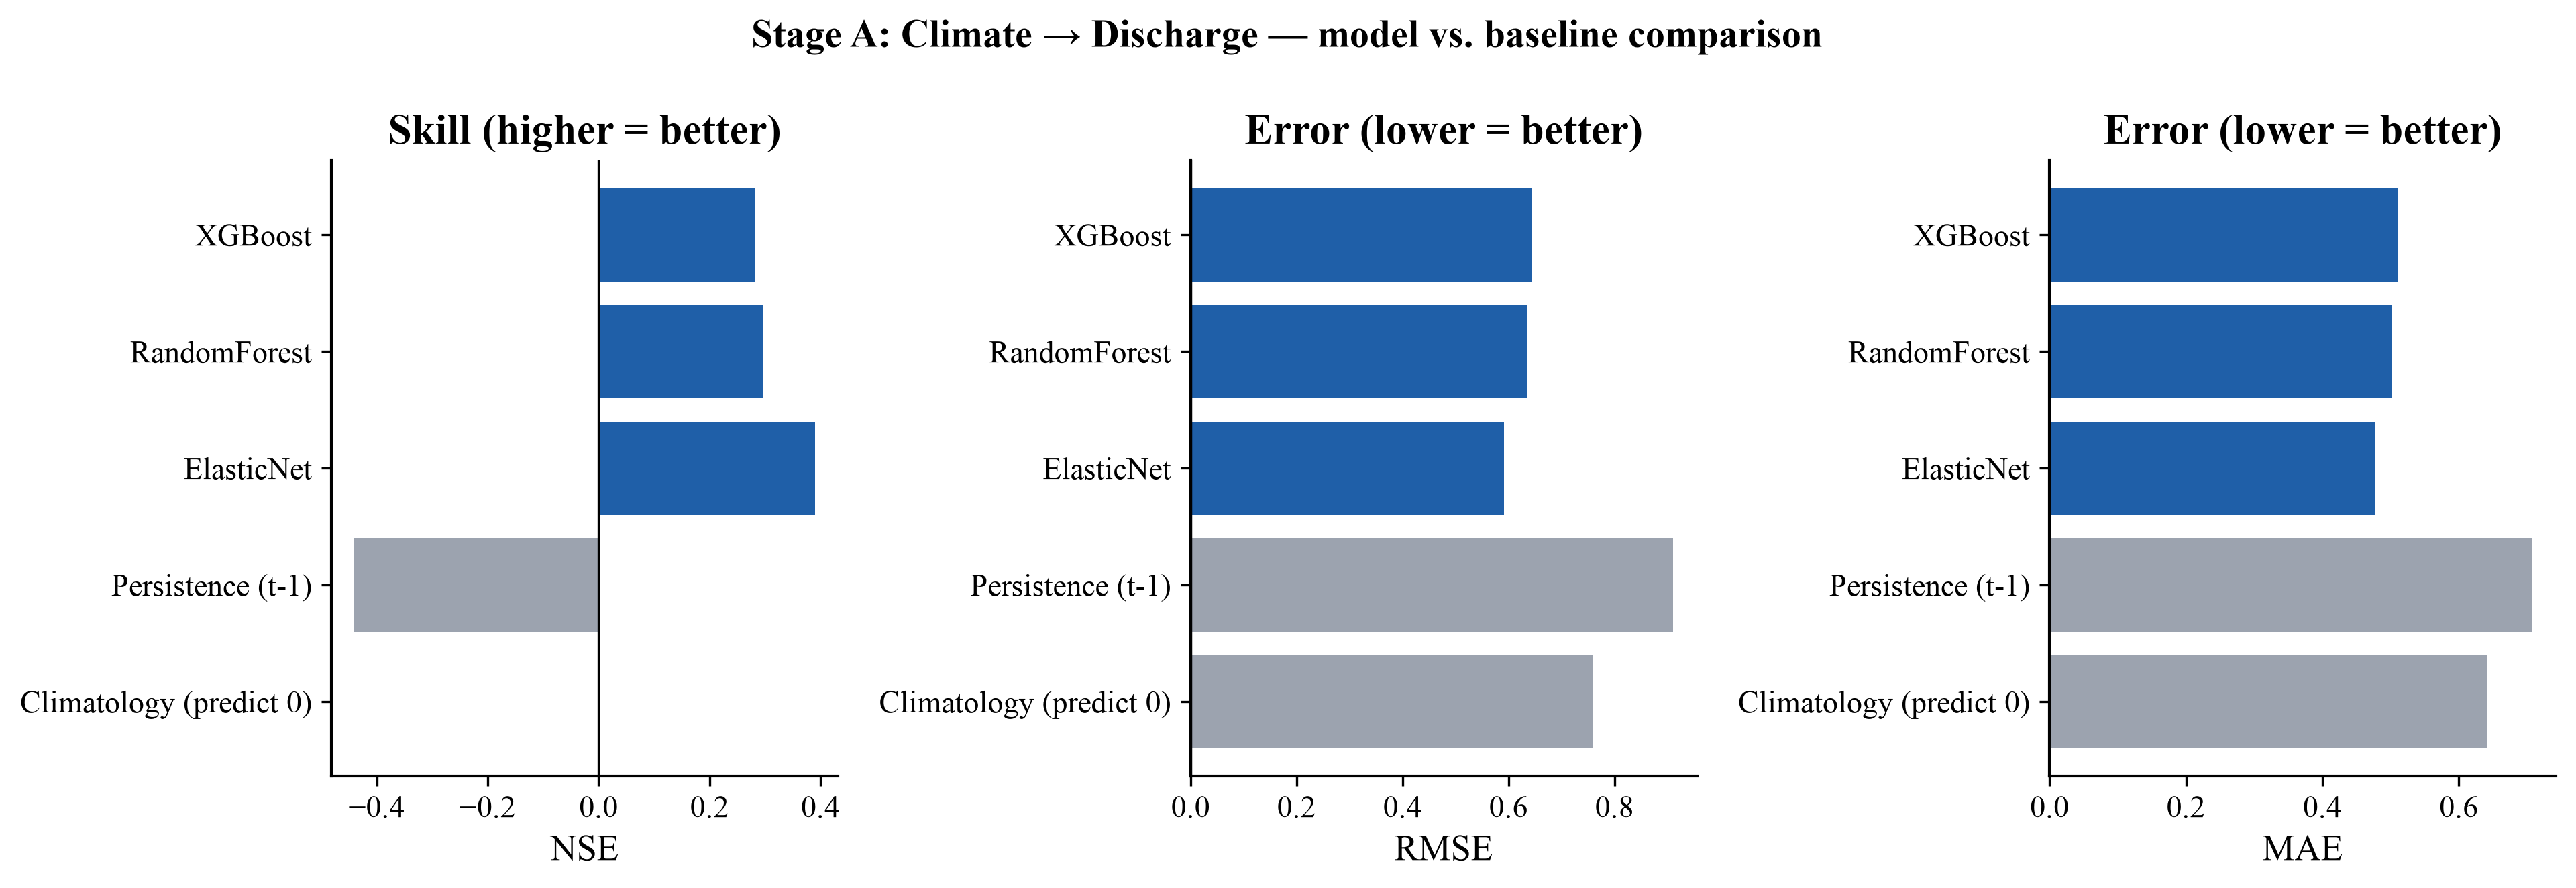
\includegraphics[width=0.9\textwidth]{../figures/11_stage_a_metrics_comparison.png}
\caption{Stage A (climate$\rightarrow$discharge) model vs. baseline comparison for the primary basin: skill (NSE) and error (RMSE, MAE).}
\label{fig:stageametrics}
\end{figure}

A common-window sensitivity analysis, restricting basins to their shared 1973--1996 period rather than each basin's own full record, confirmed that the multi-basin result is not an artifact of different basins drawing on different historical eras: all 7 basins tested under the shared window retained positive skill, though magnitudes generally shifted downward, as expected from the correspondingly smaller test sets available within that shorter window.

\subsection{Stage B: discharge-to-coastal-chlorophyll linkage in a subset of basins}
Of 7 basins with sufficient satellite-era chlorophyll-a coverage to test, 2 showed clearly positive, cross-validation-consistent skill (Loíza, Manatí; final-holdout NSE 0.03--0.15, both formally significant against the permutation null, $p=0.005$ for both; Table~\ref{tab:stageb}), 2 showed weak or mixed evidence (Patillas, Añasco), and 3 showed null or negative skill (Plata, Culebrinas, Guanajibo) under the primary merged-sensor analysis. One basin, Fajardo, could not be tested at Stage~B at all: its usable discharge record, constrained by a multi-year gap in its precipitation station (Section~2.3), ends in 1996, before the satellite ocean-color era begins, leaving no temporal overlap between the two records.

\begin{table}[htbp]
\centering
\caption{Stage B results, all 7 testable basins, final-holdout ElasticNet.}
\label{tab:stageb}
\small
\begin{tabular}{lrrrrl}
\toprule
Basin & $n_{\mathrm{test}}$ & NSE & Bias-corr. $R^2$ & Spearman $\rho$ & Verdict \\
\midrule
Loíza & 44 & 0.029 & 0.688 & --- & Confirmed \\
Manatí & 42 & 0.146 & 0.730 & 0.453 & Confirmed (less stable) \\
Patillas & 46 & 0.096 & 0.182 & 0.250 & Weak/mixed \\
Añasco & 48 & 0.063 & 0.475 & 0.544 & Weak/mixed \\
Plata & 42 & 0.030 & 0.475 & 0.233 & Null \\
Culebrinas & 45 & $-0.059$ & 0.139 & --- & Null (confound identified) \\
Guanajibo & 27 & $-0.174$ & 0.113 & --- & Null \\
\bottomrule
\end{tabular}
\end{table}

\begin{figure}[htbp]
\centering
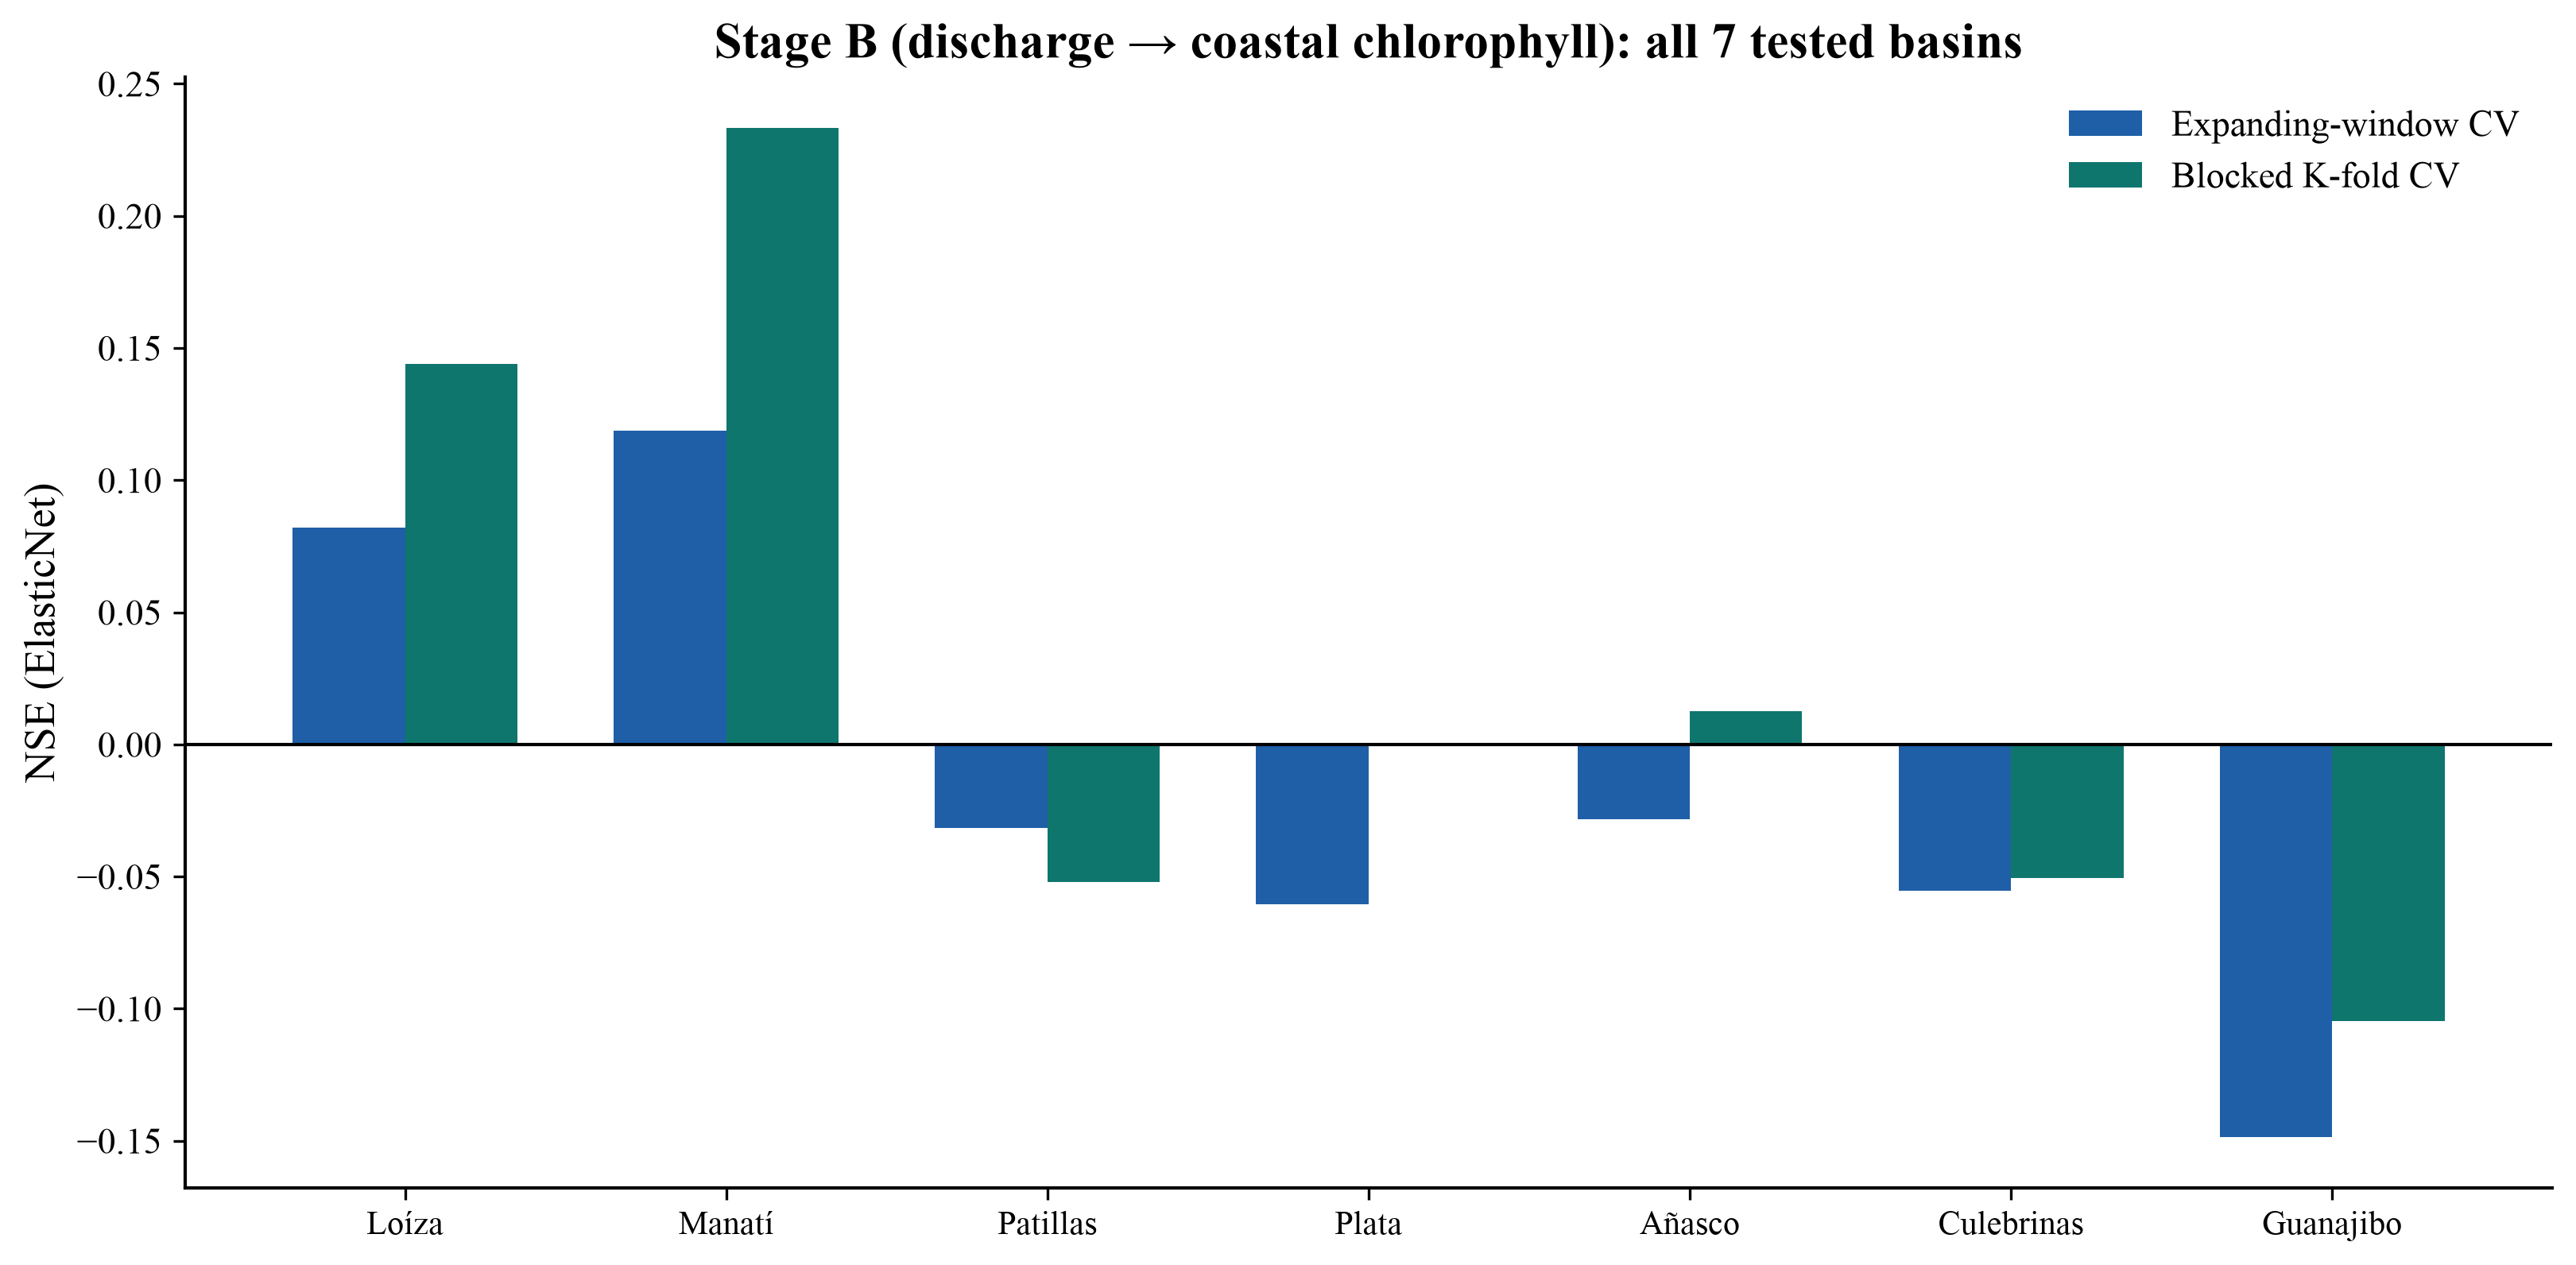
\includegraphics[width=0.9\textwidth]{../figures/14_multibasin_stage_b_comparison.png}
\caption{Stage B (discharge$\rightarrow$coastal chlorophyll) results across all 7 tested basins, both cross-validation schemes.}
\label{fig:multibasin}
\end{figure}

A learning-curve check (Fig.~\ref{fig:learning}) further distinguished the two confirmed basins from one another. Loíza's skill rose smoothly and plateaued with increasing training-set size, mirroring its Stage~A behavior. Manatí's skill was considerably less stable across training-set sizes, ranging from $-0.22$ to $+0.15$ depending on how much training data was used, before converging on its full-data value only at the largest training size tested; we therefore treat Loíza as the more robust of the two confirmed Stage~B basins and report Manatí's significance together with this stability caveat rather than as an equally solid result.

\begin{figure}[htbp]
\centering
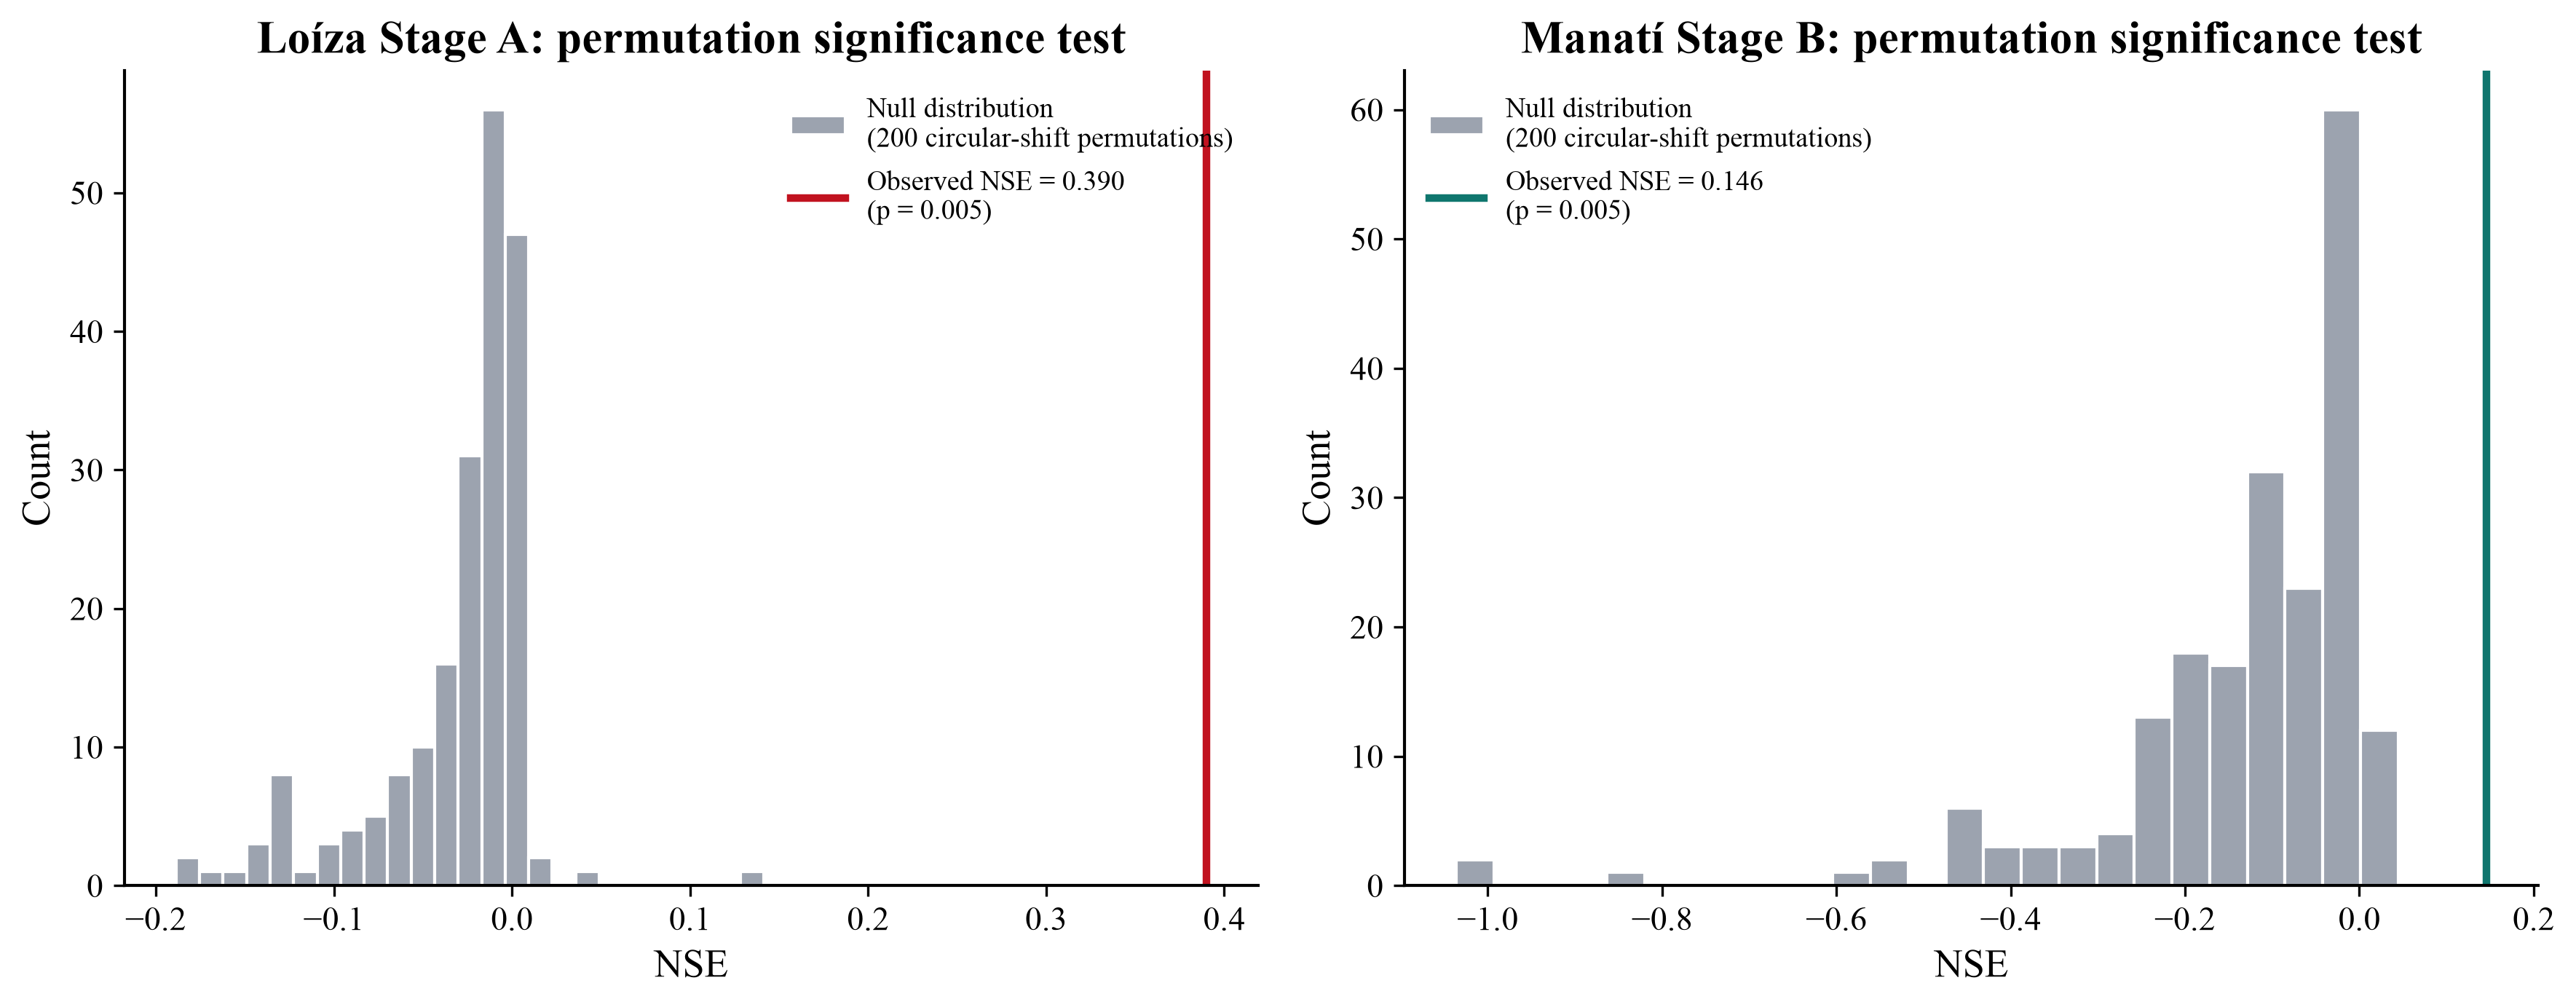
\includegraphics[width=0.85\textwidth]{../figures/20_permutation_tests.png}
\caption{Permutation significance tests for the two confirmed Stage B basins against a 200-realization circular-shift null distribution.}
\label{fig:permutation}
\end{figure}

\begin{figure}[htbp]
\centering
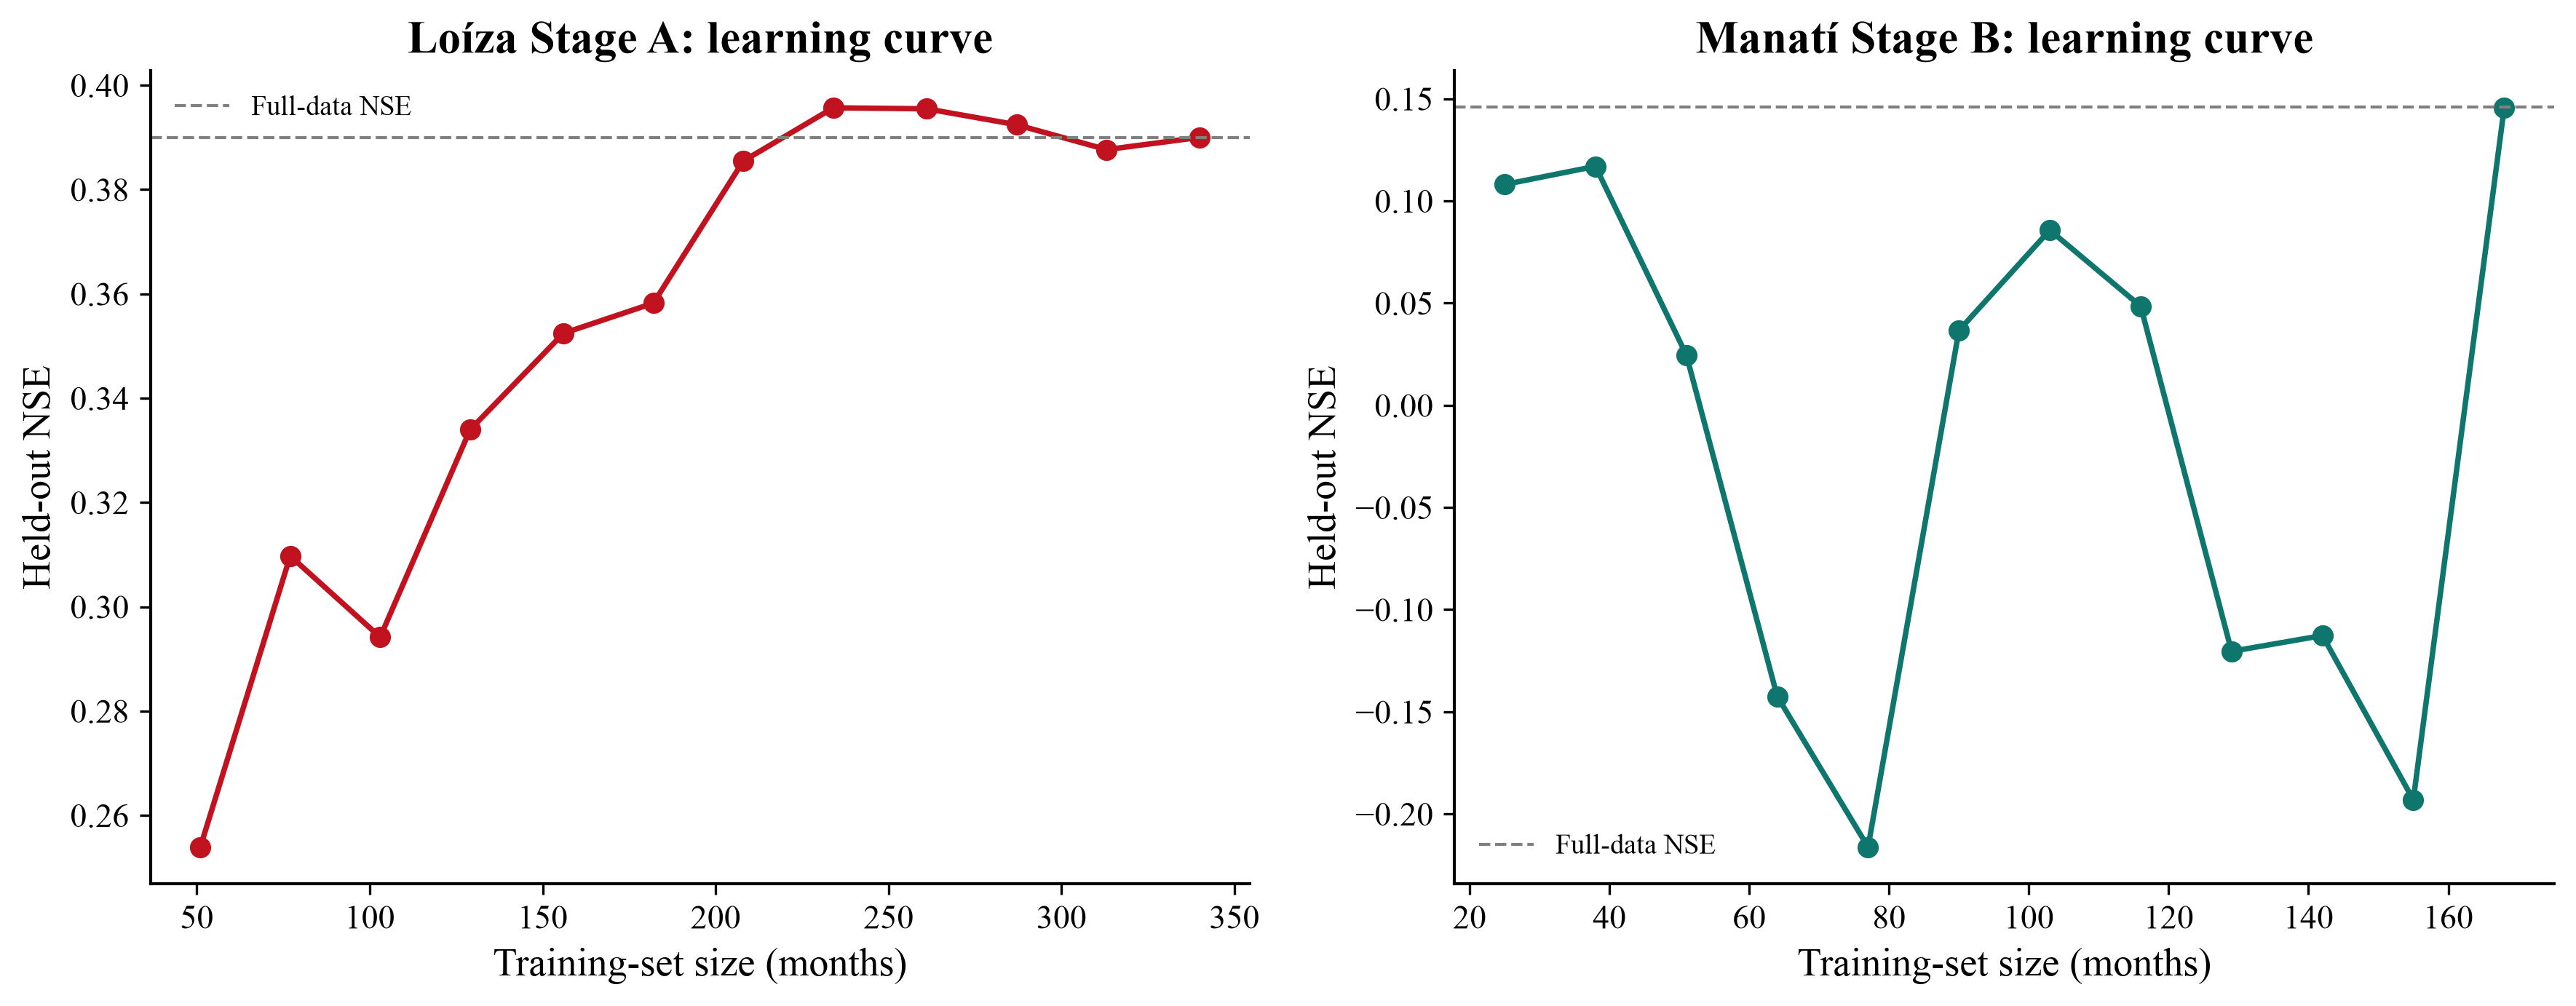
\includegraphics[width=0.85\textwidth]{../figures/21_learning_curves.png}
\caption{Learning curves (held-out NSE vs. training-set size) for the two flagship results, showing Loíza's convergence and Manatí's comparative instability.}
\label{fig:learning}
\end{figure}

SHAP attribution for both confirmed basins showed a consistent, physically coherent pattern: the same-month discharge anomaly was the dominant predictor, with contribution decaying smoothly across lags 1 through 3, and the 3-month SPI second-ranked. We view the independent reproduction of this ordered lag structure in two separate basins as evidence favoring a genuine river-to-coast transport process over a spurious statistical artifact, which would have no particular reason to reproduce a physically ordered decay pattern across basins.

Coastal box placement mattered substantially to these results. In Loíza, the offshore box outperformed the mouth-centered box (best correlation 0.50 vs. 0.23), and this offshore-favoring pattern held in 5 of 7 basins screened, consistent with the general finding of \citet{auricht2022mapping} that the discharge-chlorophyll coupling distance and lag should be characterized empirically rather than assumed. It was not universal, however: Culebrinas and Guanajibo instead favored the mouth-centered box, a difference we return to in Section~5.2.

\subsection{Explaining basin-to-basin variation in Stage B skill}
Neither drainage area nor mean discharge magnitude correlated with Stage~B skill across the 7 tested basins ($r=-0.03$ and $r=-0.04$ respectively), ruling out basin size as an explanation for which basins show a detectable coastal signal. A coastal shelf-steepness proxy, defined as the distance from the river mouth to the $-20$~m bathymetric contour, showed a moderate negative relationship ($r=-0.50$, $p=0.25$, not statistically significant at $n=7$) but was directly contradicted by Culebrinas, which had the shortest shelf distance of any basin tested yet a null result, limiting confidence in this explanation as it stands.

Investigating the Culebrinas result in more detail revealed a methodological confound rather than a purely physical one. Its final-holdout test window fell entirely within the VIIRS-only portion of the merged chlorophyll-a record, and its chlorophyll-a anomaly series showed a large discontinuity in autocorrelation structure precisely at that sensor-transition boundary (lag-1 autocorrelation 0.06 during the MODIS-covered training period versus 0.62 during the VIIRS-only test period) --- a pattern more consistent with a residual sensor-merge bias artifact than with a genuine shift in coastal chlorophyll dynamics. Culebrinas also had the weakest inter-sensor bias-correction fit of any basin ($R^2=0.14$). Testing this pattern across all seven basins, inter-sensor correction quality correlated with Stage~B skill more strongly than any physical basin characteristic examined ($r=0.66$, $p=0.11$; not statistically significant at $n=7$, but the strongest relationship found among those tested, and the only one with a clearly articulable causal mechanism connecting it to the outcome; Fig.~\ref{fig:biasr2}).

\begin{figure}[htbp]
\centering
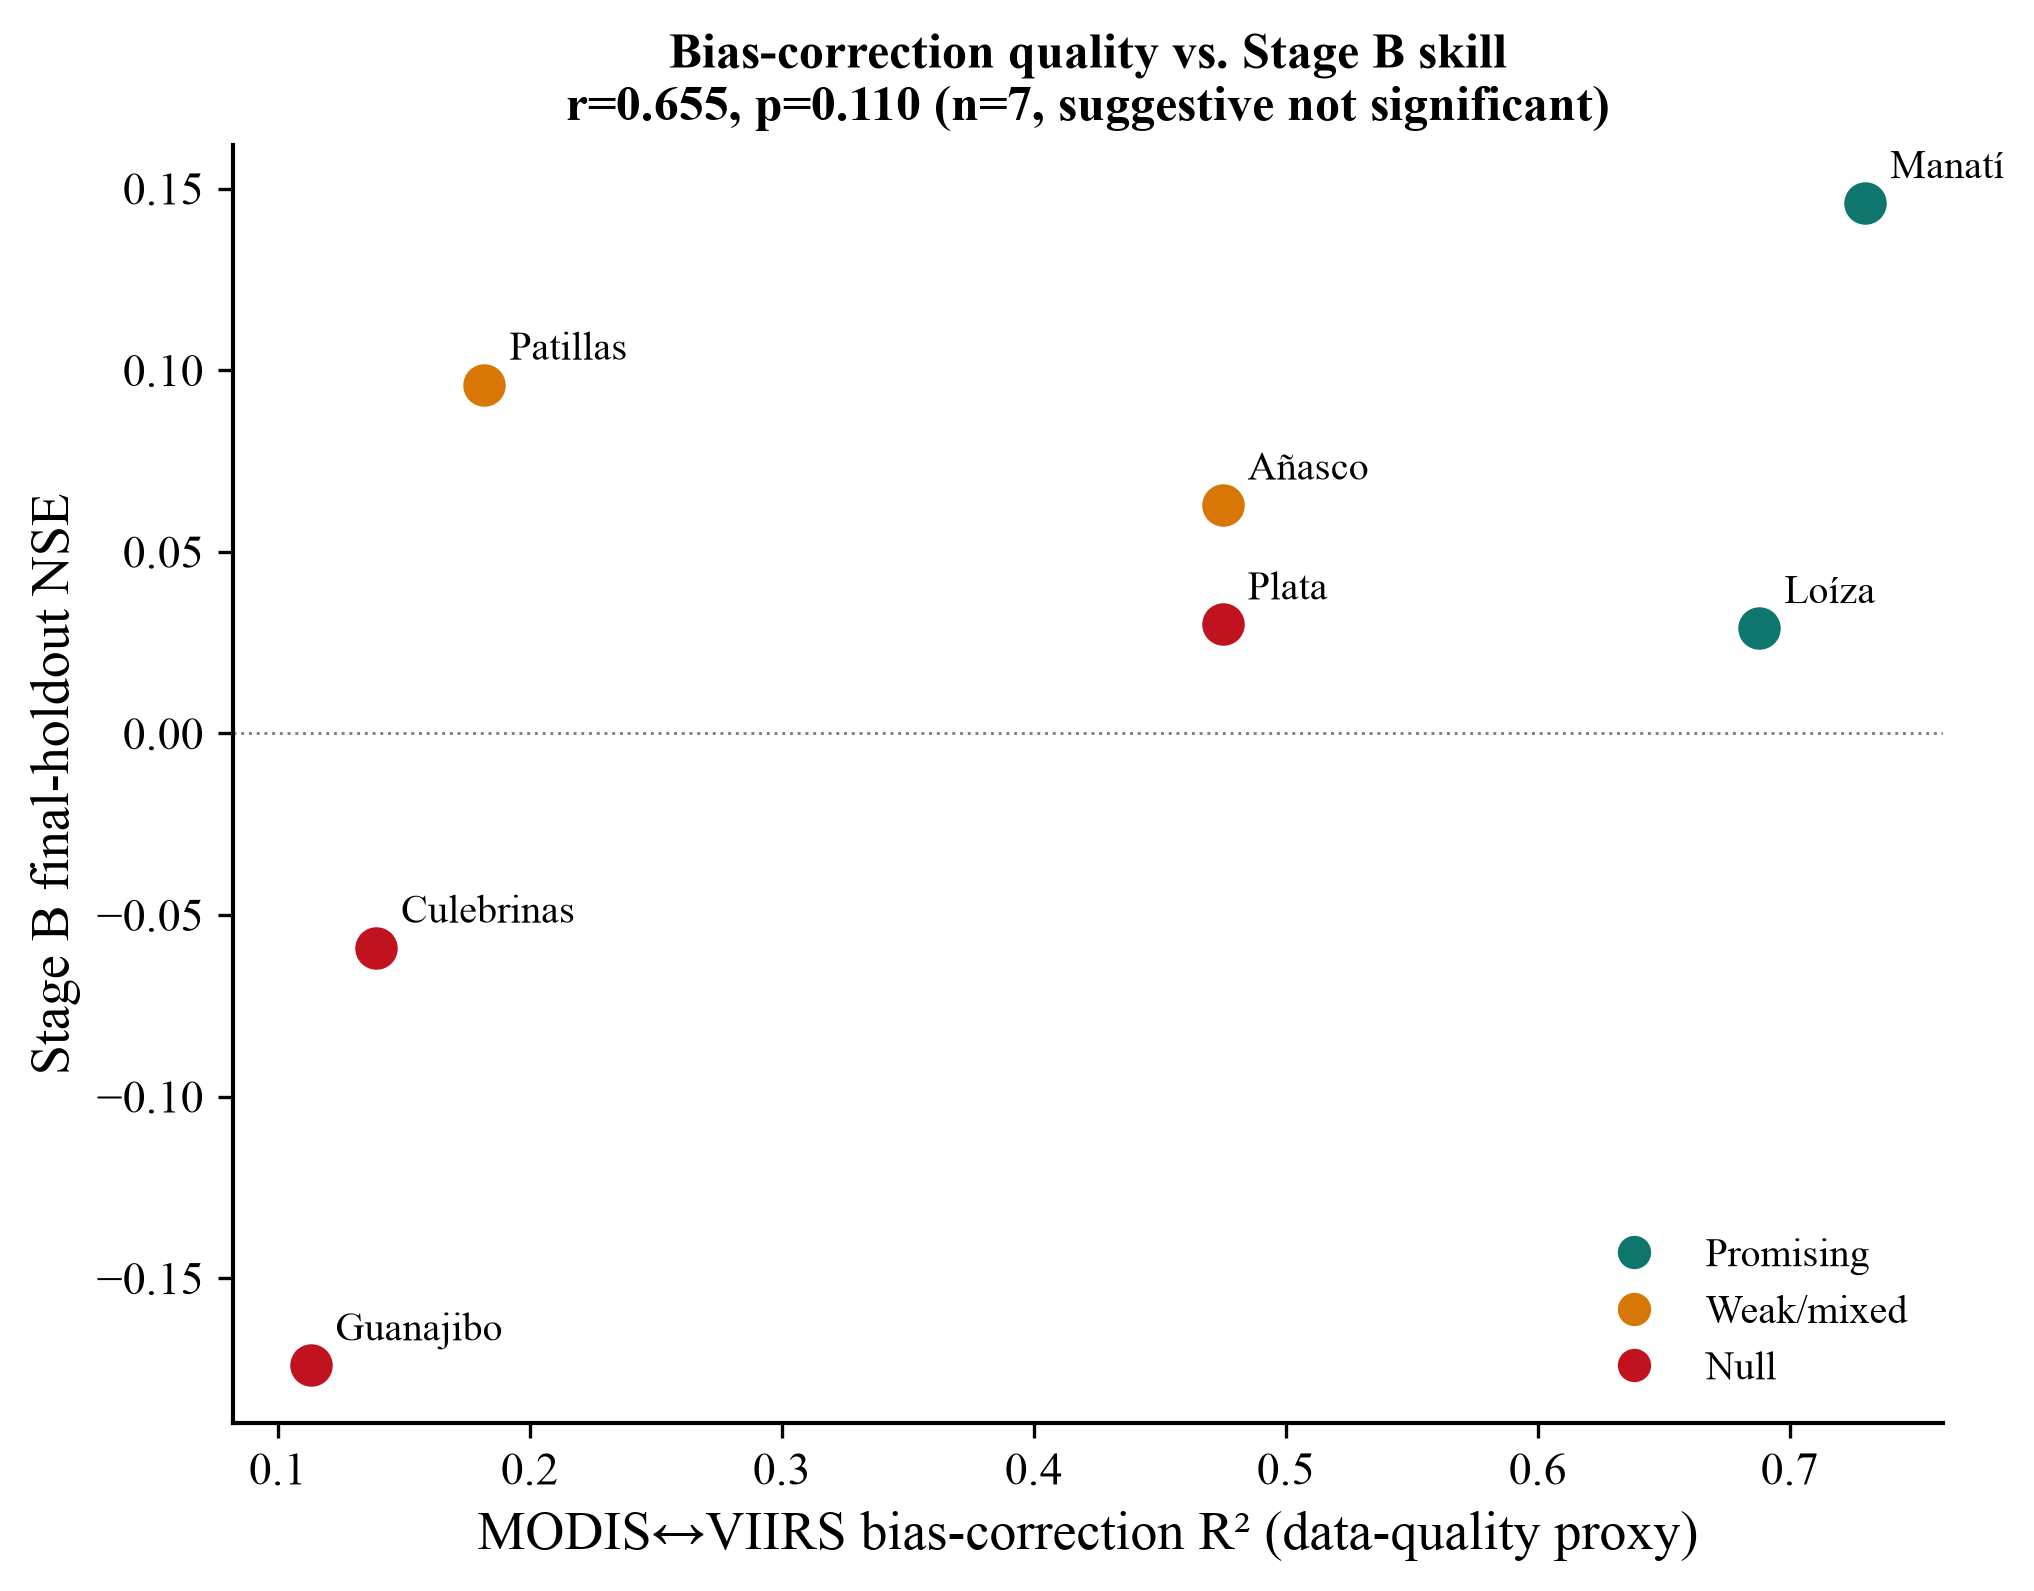
\includegraphics[width=0.7\textwidth]{../figures/18_bias_r2_vs_stage_b.png}
\caption{MODIS$\leftrightarrow$VIIRS bias-correction quality vs. Stage B skill across all 7 tested basins --- the strongest relationship found among all basin characteristics tested.}
\label{fig:biasr2}
\end{figure}

This hypothesis was tested directly, not left as a post-hoc correlation, by reprocessing the three weakest-correction basins (Culebrinas, Guanajibo, Plata) using MODIS-only data (2003--2022, with no VIIRS splice at all; Fig.~\ref{fig:modisonly}). Two of three showed the predicted improvement: Culebrinas' final-holdout NSE improved from $-0.06$ to $-0.00$, and Plata's improved from $+0.03$ to $+0.10$, with its Spearman correlation becoming clearly positive ($+0.28$), directly confirming the data-quality-confound hypothesis for those two basins. The third, Guanajibo, did not improve ($-0.17$ to $-0.20$), suggesting that its null result more likely reflects either a genuine absence of a detectable coastal linkage or a sample-size limitation --- its 27-month test period was the shortest of any basin studied --- rather than the same sensor-merge artifact.

\begin{figure}[htbp]
\centering
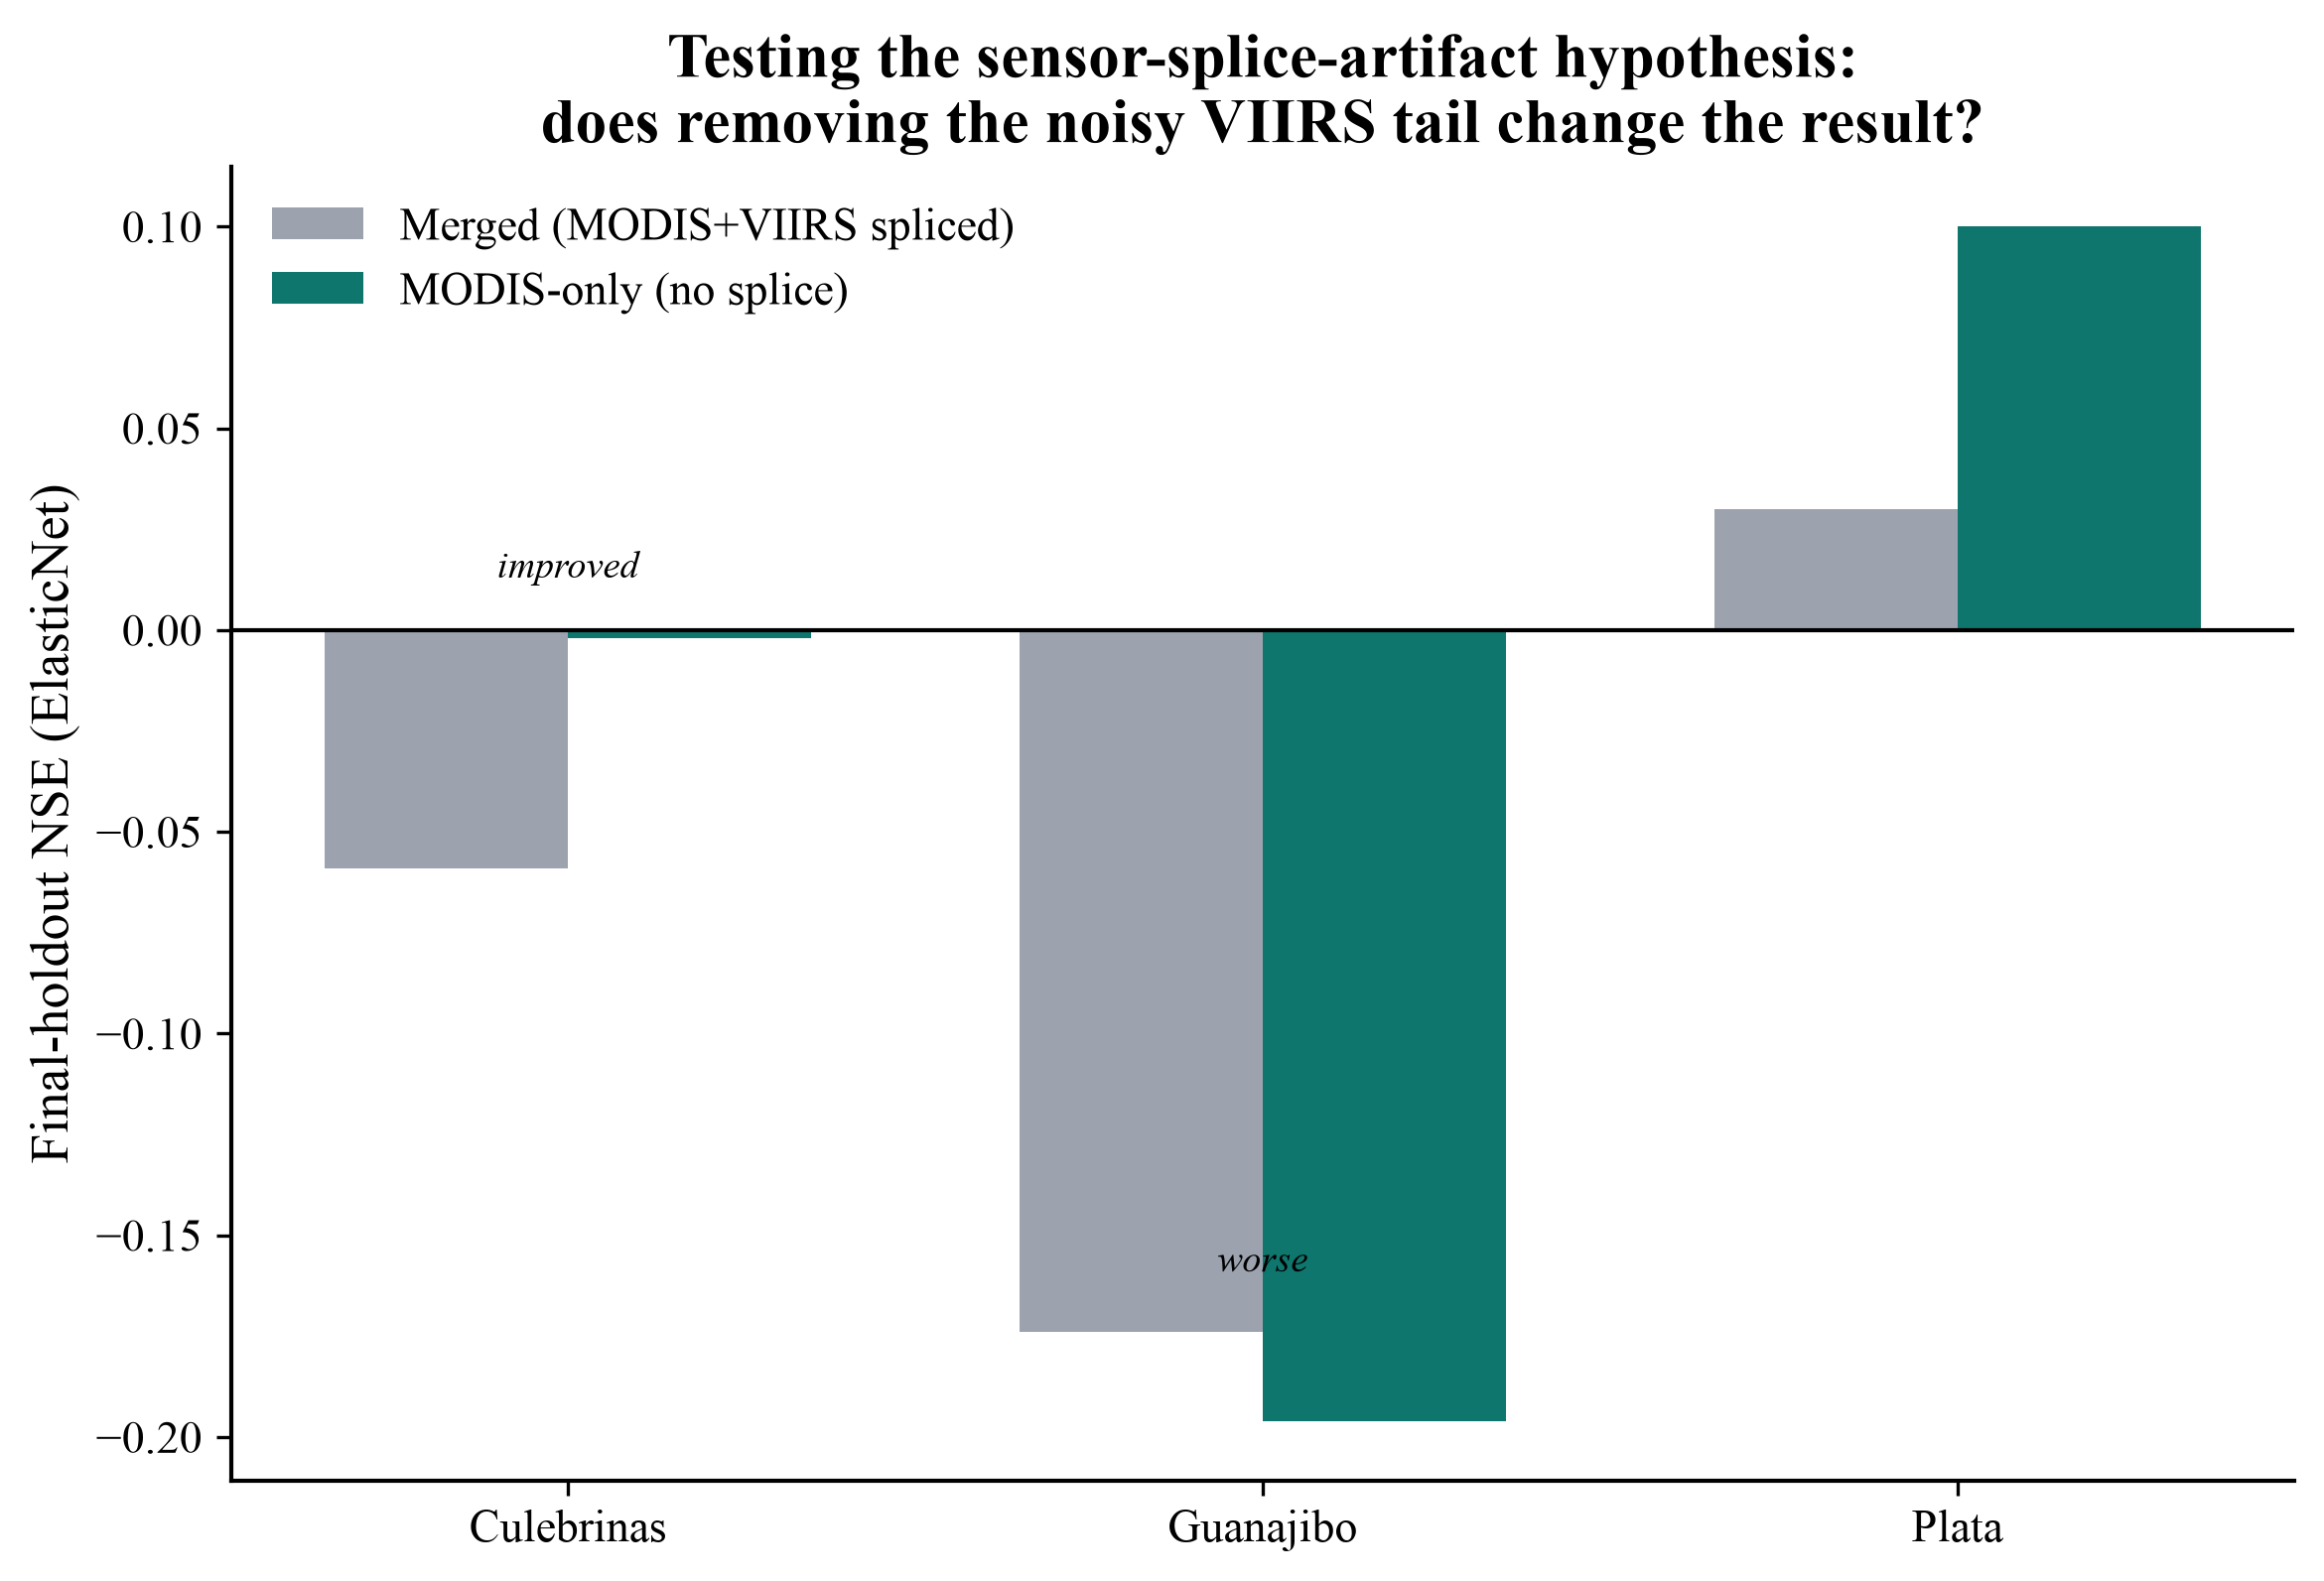
\includegraphics[width=0.8\textwidth]{../figures/19_modis_only_retest.png}
\caption{Direct test of the sensor-splice-artifact hypothesis: final-holdout NSE for the three weakest-correction basins under the original merged (MODIS+VIIRS) data vs. MODIS-only data.}
\label{fig:modisonly}
\end{figure}

\section{Discussion}

\subsection{Significance and novelty}
This study's central contribution is methodological as much as it is a specific set of basin results: it demonstrates, with direct empirical tests rather than assertion, that (i) a climate-discharge relationship in a tropical small-island setting can be shown to generalize across basins rather than remaining a single-watershed finding, (ii) a discharge-coastal-chlorophyll linkage, where present, can be attributed to a specific driver and lag using an explainable framework rather than reported only as a bulk accuracy number, and (iii) apparent cross-basin heterogeneity in such a linkage can itself be partially explained and, where a data-quality mechanism is suspected, directly tested rather than left as an unexplained residual. To our knowledge, no prior study of Puerto Rico's climate-discharge-coast chain has combined a multi-basin design with this level of statistical validation (two independent cross-validation schemes, permutation-based significance testing, block-bootstrap confidence intervals, and learning-curve stability checks) or has identified and directly confirmed a satellite-sensor-merging confound as a partial explanation for cross-basin null results. This last point extends beyond Puerto Rico: it is directly relevant to any study that merges a heritage ocean-color sensor (such as MODIS) with a current one (such as VIIRS or a future successor) for a discharge or land-margin analysis, and it echoes, from a different angle, the broader finding of \citet{holbach2025chlorophyll} that a satellite chlorophyll-a product's reliability is not uniform across space and should be checked rather than assumed --- in their case through spatial recalibration of the retrieval algorithm itself, and in ours through a per-basin diagnostic of inter-sensor agreement.

\subsection{On generalization and the offshore-versus-mouth finding}
The Stage~A result --- climate-driven discharge predictability across all 10 tested basins, formally significant at the primary basin, and physically coherent in its SHAP attribution --- is this study's most robust finding and directly answers a question that a single-basin pilot study cannot: whether an observed climate-discharge relationship is a general feature of Puerto Rico watersheds or an artifact of one basin's particular characteristics. The Stage~B result is deliberately reported as heterogeneous rather than forced into a uniform positive or uniform null conclusion, which we regard as more scientifically honest and more useful to future work, since it identifies not only where a linkage is detectable but, for a subset of basins, why it is or is not. That coastal chlorophyll response peaks offshore rather than at the point of discharge in most, but not all, basins tested is consistent with the broader river-plume literature, in which surface chlorophyll signatures build as freshwater disperses and mixes rather than peaking at the point source \citep{auricht2022mapping}. A denser spatial search than the two-candidate screen used here would be needed to map this offshore distance precisely across basins, and we treat the present finding as a first-order empirical result motivating that follow-up rather than as a settled spatial rule.

\subsection{Limitations}
Several limitations bound the interpretation of these results. Basin sample size ($n=7$--10, depending on stage) is adequate to demonstrate that the Stage~A climate-discharge relationship generalizes across independent basins, but it is not adequate to statistically confirm the Stage~B basin-characteristic explanations explored in Section~4.3, which remain suggestive ($p>0.05$ throughout) rather than confirmed; a substantially larger basin sample, or an alternative analysis pooling basins directly rather than comparing basin-level summary statistics, is identified as necessary future work. Coastal box placement, while empirically tested at each basin rather than assumed uniformly, was tested at only two candidate positions per basin, so the reported offshore distances should be read as a first approximation rather than a precisely mapped optimum. The Manatí Stage~B result, while formally significant on the full dataset, showed materially less stability across training-set sizes than the Loíza result and should be weighted accordingly in any synthesis across the two confirmed basins. Finally, the satellite-sensor-merging confound identified in Section~4.3 was tested for only three basins; whether it explains additional variance among the basins not directly retested (Patillas, Añasco) is not established here.

\section{Conclusion}
This study provides multi-basin, statistically tested, and physically interpretable evidence that local drought conditions, rather than ENSO, drive river discharge variability across Puerto Rico watersheds (H1), confirmed in all 10 basins tested; that a discharge-to-coastal-chlorophyll linkage is detectable in a subset of basins and is concentrated offshore rather than at the river mouth in most cases (H2); and that an explainable machine-learning framework can both quantify this skill and diagnose why it is or is not detected in a given basin, including identifying and partially confirming a satellite-sensor-merging data-quality confound (H3). These findings extend prior single-basin and single-event work in Puerto Rico to a systematic, generalizable, and self-critically validated multi-basin assessment, and they identify a concrete, transferable data-quality consideration for future satellite-based coastal monitoring studies in small tropical-island systems more broadly.

\section*{Data and Code Availability}
All data used are from public sources: USGS NWIS, NOAA GHCN-D, NOAA CoastWatch ERDDAP (MODIS and VIIRS chlorophyll-a, OISST), NCEP/NCAR Reanalysis, USGS NHD, OpenStreetMap, UN OCHA COD-AB, and GEBCO. Analysis code is available at [repository URL to be added prior to submission].

\section*{CRediT Authorship Contribution Statement}
\textbf{Somnath Luitel:} Conceptualization, Methodology, Software, Formal analysis, Data curation, Writing -- original draft, Visualization. \textbf{Manmeet Singh:} Conceptualization, Supervision, Writing -- review \& editing.

\section*{Declaration of Competing Interest}
The authors declare no competing financial interests or personal relationships that could have influenced the work reported in this paper.

\bibliographystyle{elsarticle-harv}
\bibliography{references}

\end{document}
